\chapter{Parallel Computing}
%\vspace{10.5cm}
\vfill
Per realizzare gli appunti su questa parte del corso, ho usato le slides del prof. Gianluca Lamanna disponibili su e-learning.

\newpage
\section{\textit{Gio 20 ott - Lezione 9}}
\section{Computer architecture from a
performance point of view: from
serial to parallel}
\sectionmark{from
serial to parallel}

\subsection{Architettura di Von Neumann}
L'architettura di Von Neumann è una tipologia di architettura hardware per computer digitali programmabili a programma memorizzato la quale condivide i dati del programma e le istruzioni del programma nello stesso spazio di memoria, contrapponendosi all'architettura Harvard nella quale invece i dati del programma e le istruzioni del programma sono memorizzati in spazi di memoria distinti. 
Introdotta nel 1945 da John Von
Neumann, consiste di 5 elementi:
\begin{enumerate}
    \item Processing unit (arithmetic logic
unit)
    \item Control unit (instruction pool)
    \item Memory
    \item Bus
    \item I/O
\end{enumerate}

\begin{figure}[ht]
    \centering
    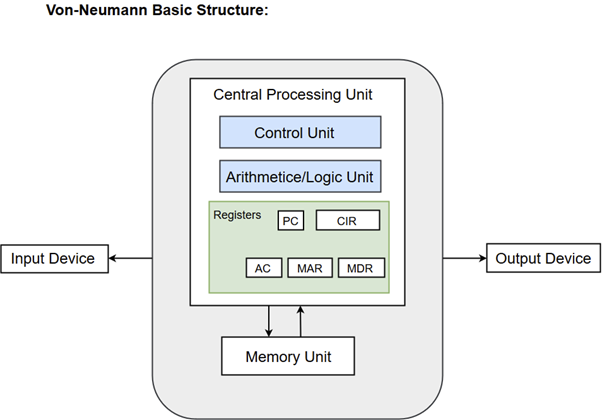
\includegraphics[width=0.6\textwidth]{figure_parallel/VN_arch.png}
\end{figure}
\FloatBarrier


Da una parte abbiamo i dati, dall'altra abbiamo i programmi. La parte di controllo copia i dati dalla memoria in una memoria temporanea e vi esegue i comandi contenuti nei programmi.\\

\subsection{Von Neumann Bottleneck}
L'architettura di Von Neumann presenta delle limitazioni legate al fatto che viene condiviso lo stesso bus per dati e istruzioni, creando il cosiddetto \textit{Von Neumann Bottleneck}.\\



\begin{figure}[ht]
    \centering
    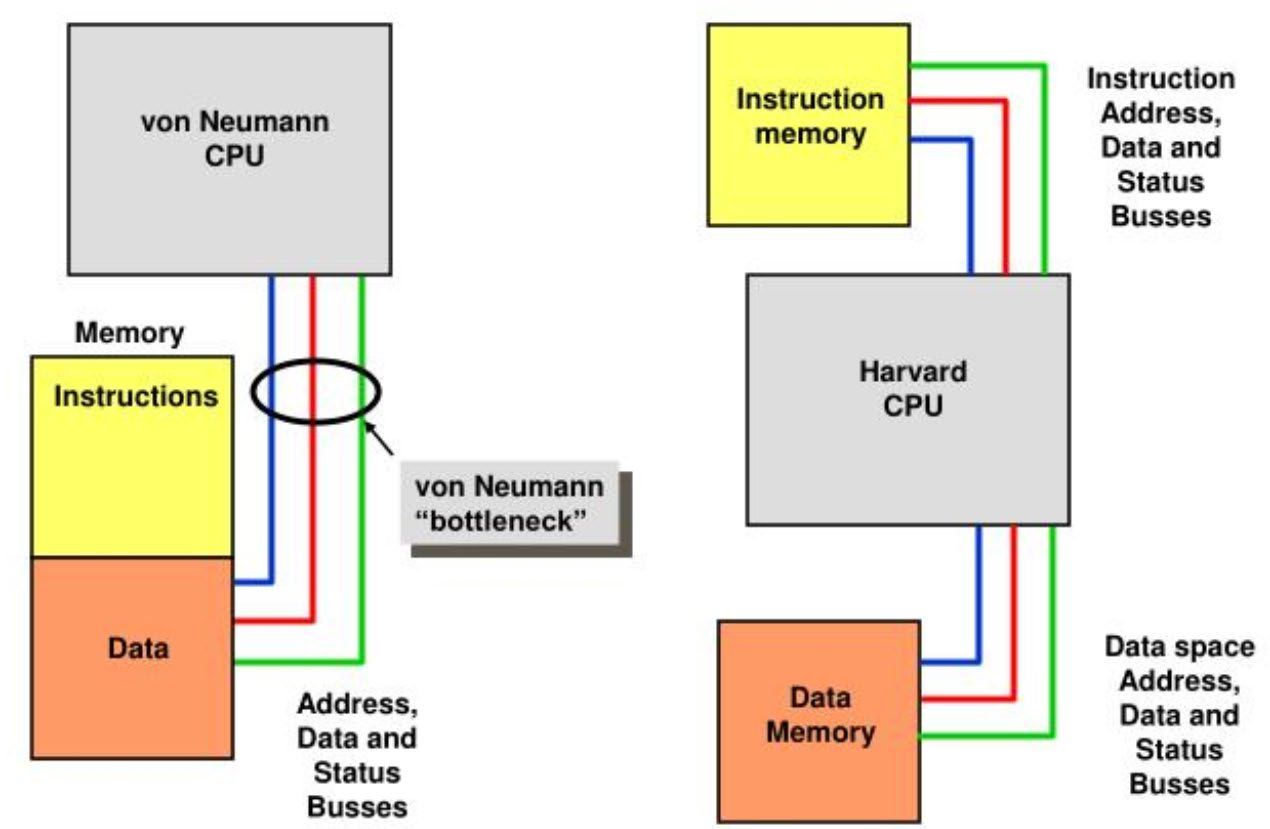
\includegraphics[width=0.6\textwidth]{figure_parallel/bottleneck.png}
\end{figure}
\FloatBarrier


Esistono varie strategie per mitigare questo fenomeno:
\begin{enumerate}
    \item Caching and memory gerarchy on chip
    \item Separate access to data and instructions (Harvard Architecture)
    \item Branch prediction
\end{enumerate}

\subsection{Simple Server architecture}
In a server multiple components interacts during the program execution.
\begin{itemize}
    \item Processors/cores
    \begin{itemize}
        \item I-cache, D-cache
    \end{itemize}
    \item Shared Caches
    \begin{itemize}
        \item For instruction and data
    \end{itemize}
    \item Memory controllers
    \item I/O subsystems
        \begin{itemize}
        \item Storage, network, peripherals
    \end{itemize}
\end{itemize}

\begin{figure}[ht]
    \centering
    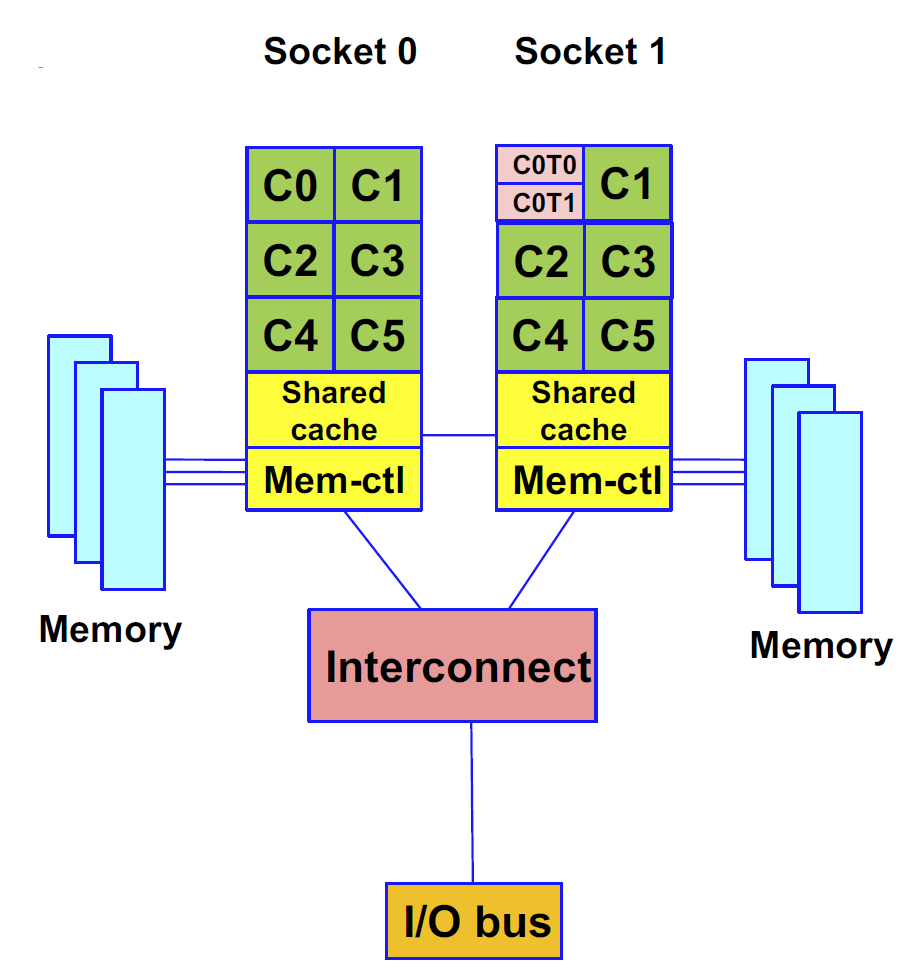
\includegraphics[width=0.5\textwidth]{figure_parallel/server.png}
\end{figure}
\FloatBarrier

An example: NUMA architecture (non-
uniform memory access).

\subsection{Memoria}
Ci sono 2 parametri che caratterizzano le memorie:\\ 
\textbf{Banda:} numero di byte che posso estrarre dalla memoria ad ogni colpo di clock.\\
\textbf{Latenza:} quanto tempo ci vuole dopo che abbiamo richiesto i dati ad ottenerli effettivamente.\\

Se ho un'operazione che eseguo molto spesso, non conviene ogni volta accedere a questa operazione.
Analogamente, se abbiamo gli stessi dati su cui fare delle operazioni, li carichiamo nella cache una volta sola e poi facciamo le operazioni.\\

In particolare, la cache è strutturata su più livelli, ognuno dei quali ha performance diverse in termini di Banda e Latenza.\\
La gerarchia di "data access" e "instruction fetching" è fondamentale nell'architettura dei computer.\\

\begin{figure}[ht]
    \centering
    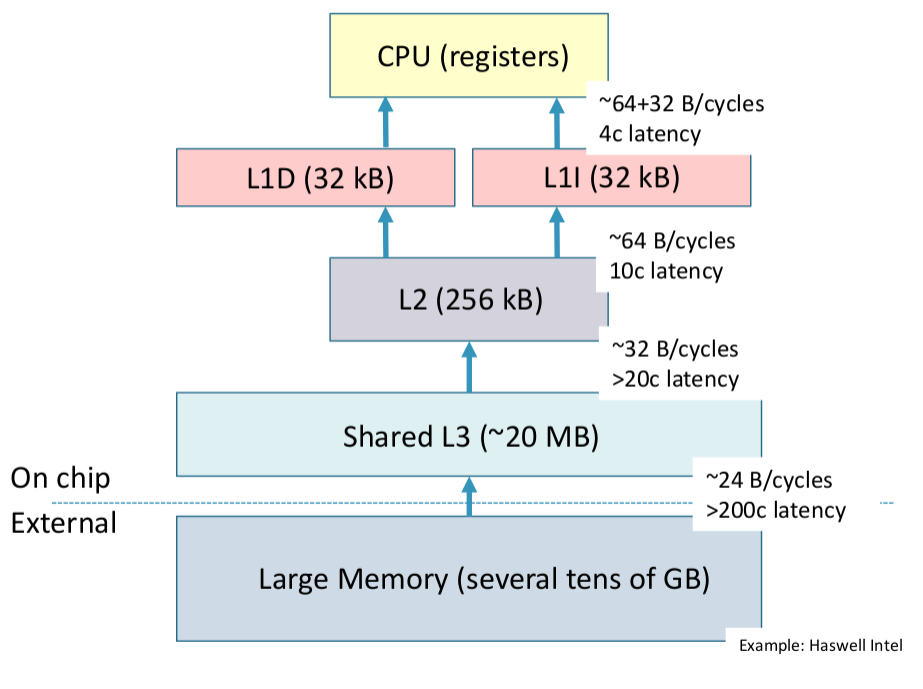
\includegraphics[width=0.6\textwidth]{figure_parallel/cache.png}
\end{figure}
\FloatBarrier

Più il clock va veloce e più il processore è veloce. Tuttavia la velocità del clock non può aumentare all'infinito. Si cercano metodi per andare più veloci del tempo scandito dal clock.\\

\subsection{Seven dimensions of performance}
The «modern» PC performance depends on (at least) seven characteristics:

\begin{figure}[ht]
    \centering
    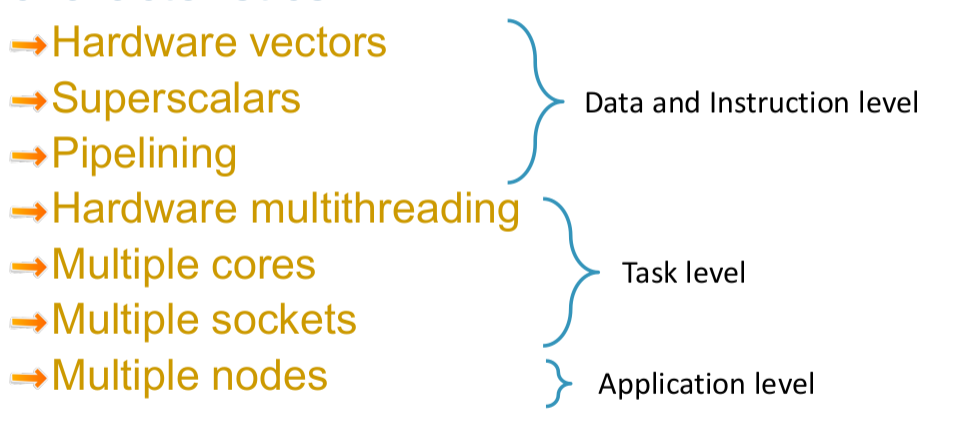
\includegraphics[width=0.6\textwidth]{figure_parallel/7perf.png}
\end{figure}
\FloatBarrier

\subsection{Processori Vettoriali}
Finora abbiamo visto processori "scalari".\\
Modern processors implement registers for vectorialization (SSE/SSE2 and
AVX)

\begin{itemize}
    \item Scalar mode:
    \begin{itemize}
        \item One operation produces one result
    \end{itemize}
    \item SIMD (Single Instruction Multiple Data) is a simple way to parallelize
    \begin{itemize}
        \item One operation produces multiple results
    \end{itemize}
\end{itemize}

\begin{figure}[ht]
    \centering
    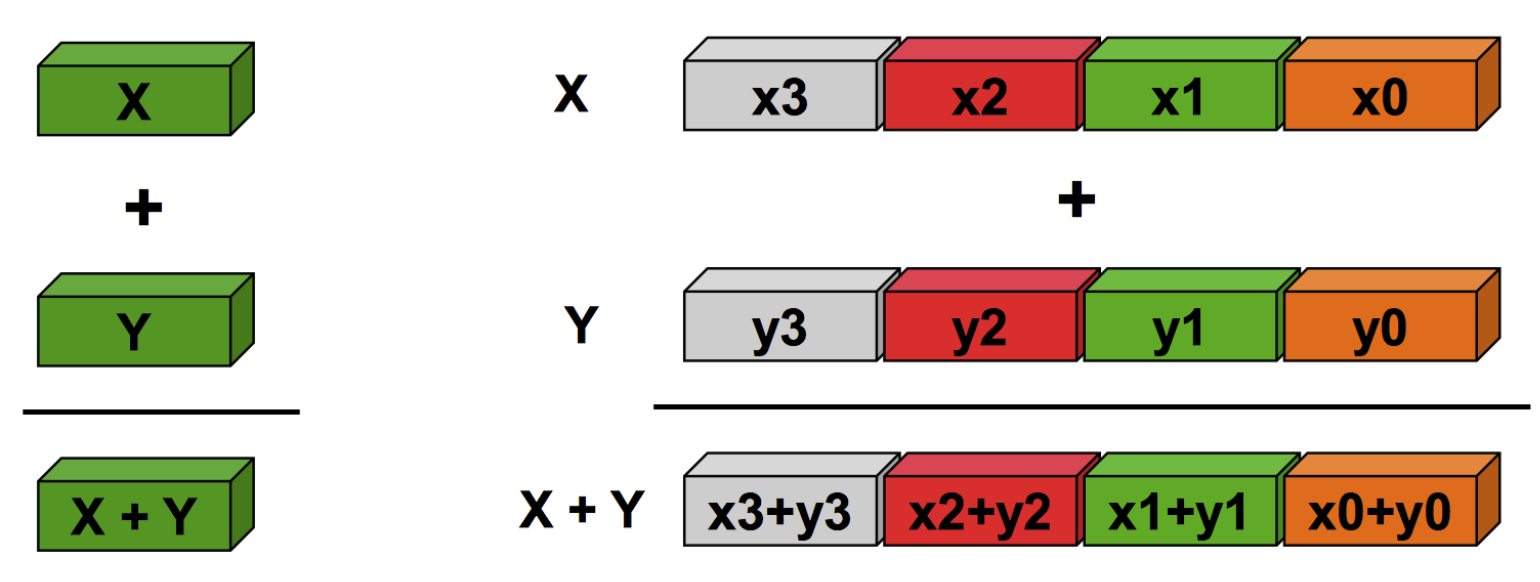
\includegraphics[width=0.7\textwidth]{figure_parallel/vector_sum.png}
\end{figure}
\FloatBarrier

\subsection{Superscalari}
Abbiamo tanti processori scalari, ognuno dei quali fa singole operazioni su singoli elementi di memoria. \\

\begin{figure}[ht]
    \centering
    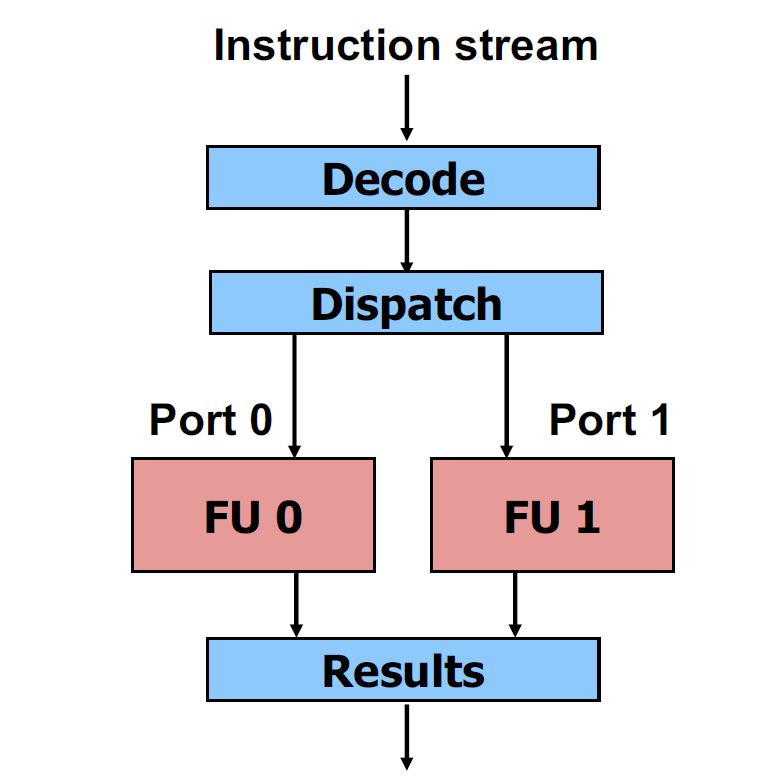
\includegraphics[width=0.4\textwidth]{figure_parallel/superscalar.png}
\end{figure}
\FloatBarrier

\begin{itemize}
    \item Architecture between pure «scalar» and pure «vector»
    \begin{itemize}
        \item Several hardware units can execute different operation on different data at the same time
    \end{itemize}
\end{itemize}




\begin{itemize}
    \item Functional Units (FU) can have identical or different computing capabilities
    \begin{itemize}
        \item Decoder and Dispatcher must have the capability to manage two instruction in one clock cicle
    \end{itemize}
\end{itemize}

\begin{itemize}
    \item Usefull for Branch Prediction
    \begin{itemize}
        \item Execute at the same time different branches in an algorithm then choose the correct one
    \end{itemize}
\end{itemize}



\textbf{Branch prediction}:
Ho sufficienti risorse per eseguire contemporaneamente varie branch di un programma.

\subsection{Pipelining}


Pipelining consists in the capability to execute different stage of consecutive instructions at the same time.

\begin{figure}[ht]
    \centering
    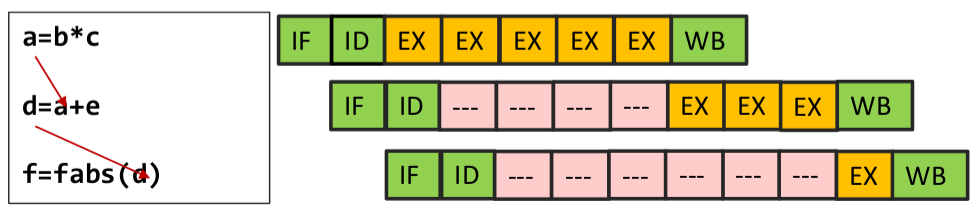
\includegraphics[width=0.7\textwidth]{figure_parallel/pipeline.png}
\end{figure}
\FloatBarrier

The pipeline is an important ingredient in
modern processors. However, it isn’t always possible to fully exploit the pipeline.

\begin{figure}[ht]
    \centering
    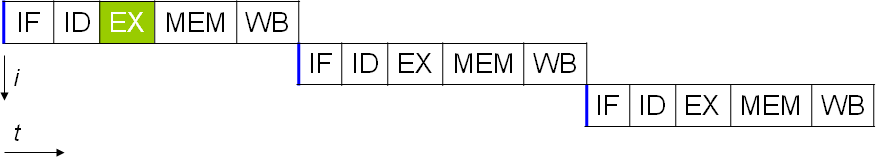
\includegraphics[width=0.5\textwidth]{figure_parallel/pipeline1.png}
    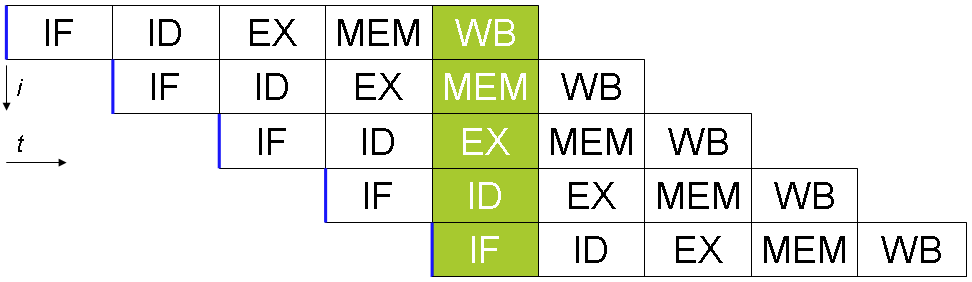
\includegraphics[width=0.5\textwidth]{figure_parallel/pipeline2.png}\end{figure}
\FloatBarrier


\begin{tcolorbox}[width=\textwidth,colback={white},title={Summary: },colbacktitle=cyan,coltitle=black]
  \begin{itemize}
    \item Superscalars, Pipelining and Vectorialization are methods to exploit some «parallelism» at the instruction and data level: ILP
    \begin{itemize}
        \item Probably OOO (Out-of-order) execution should be included in this category
    \end{itemize}
    \item The possible improvement thanks to ILP depends on problem and data structures
    \begin{itemize}
        \item 1x-10x for Superscalars and Pipeline
        \item 2x,4x,8x,16x for the vectorialization
    \end{itemize}
    \item These methods show «saturation» because they are limited by the CPU resources available
        \begin{itemize}
        \item Pentium 4: 30 pipeline stages (nowadays 10-15 maximum)
        \item ARM A57 (Apple A7/A8): 9 ports/6 instructions superscalar
        \item Intel Tiger Lake: vector of 512 bits for a subset of AVX512 instructions
    \end{itemize}
   \end{itemize}  
   … the point is: can CPU resources grow indefinitely?
\end{tcolorbox}


\subsection{Dennard Scaling}

\begin{wrapfigure}{r}{0.4\textwidth}
  \begin{center}
    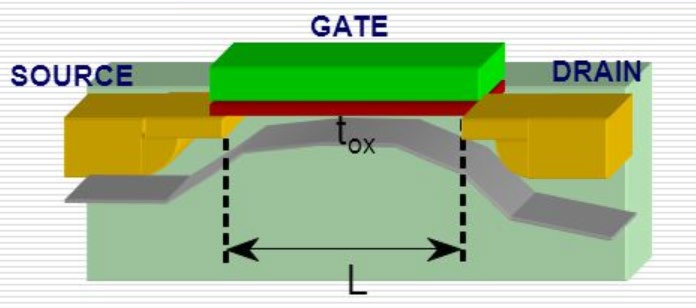
\includegraphics[width=0.35\textwidth]{figure_parallel/fet.png}
  \end{center}
\end{wrapfigure}

Aka MOSFET scaling (Dennard scaling after an article from Dennard et al. in 1974 in IEEE Journal of Solid State Circuits)\\
\textbf{-In each generation of CMOS based IC the power
consumption remains the same}\\
Breakdown of Dennard scaling around 2006: With very small integration it is not true anymore that the power consumption is the same, due to increasing in current leakage. The increasing of the speed of the transistors switching (frequency) is not anymore linear with the performance of the CPU\\

Energy consumption has become more important to users (For mobile, IoT, and for large clouds).\\
Processors have reached their power limit: Thermal dissipation is maxed out (chips turn off to avoid
overheating!). Even with better packaging: heat and battery are limits.

\begin{figure}[ht]
    \centering
    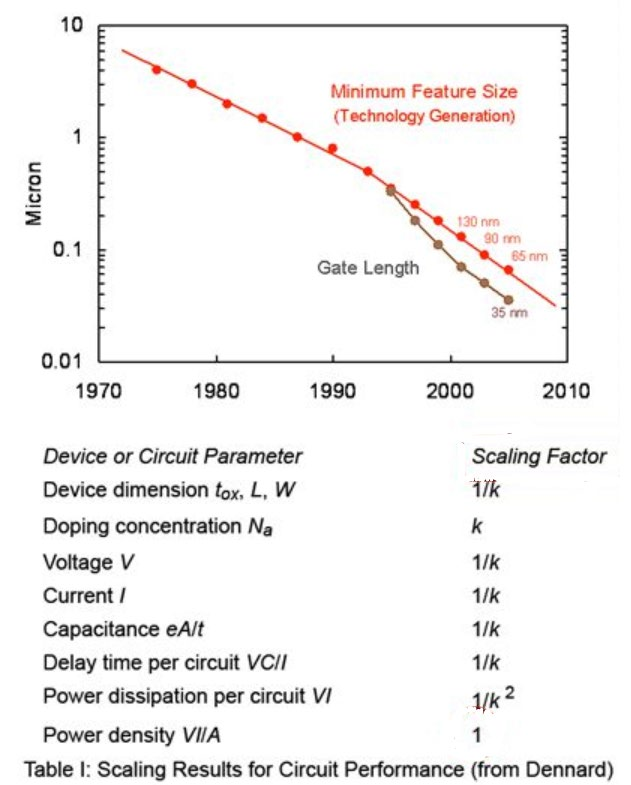
\includegraphics[width=0.4\textwidth]{figure_parallel/dennard.png}\end{figure}
\FloatBarrier

\subsection{Moore scaling}


Moore’s «law» is the empirical
observation that the number of
transistors doubles about each two
years (the performance of CPU doubles each 18 months).\\
Moore’s prediction was verified for
decades, however, around 2005 is starts to show saturation!\\
Moore's law is closely related to Dennard scaling.


\begin{figure}[ht]
\centering
\begin{subfigure}{.5\textwidth}
  \centering
  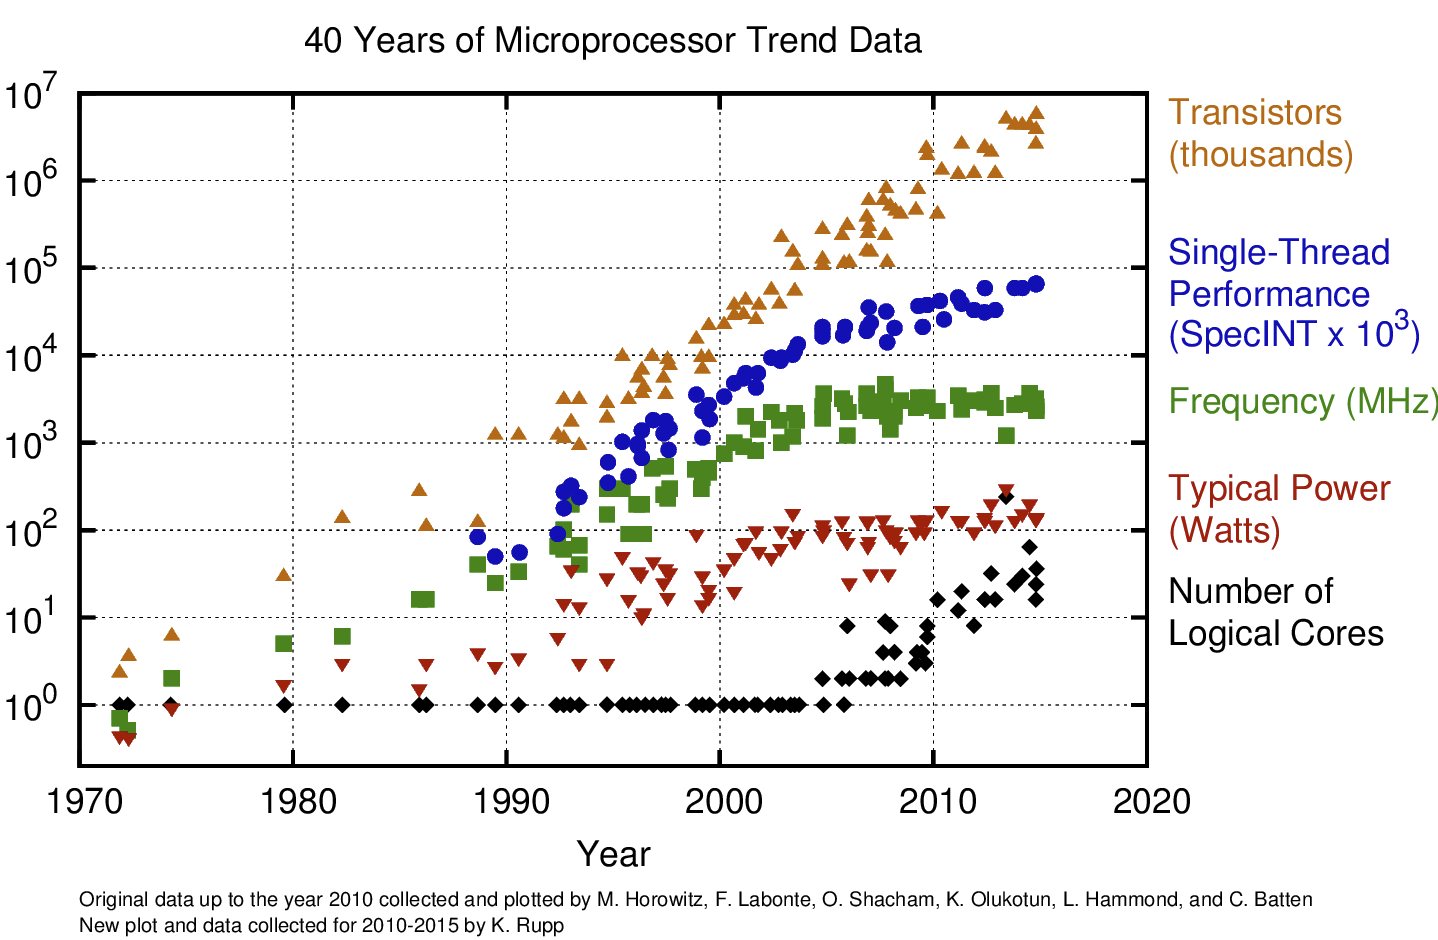
\includegraphics[width=.9\textwidth]{figure_parallel/moore.png}
\end{subfigure}%
\begin{subfigure}{.5\textwidth}
  \centering
  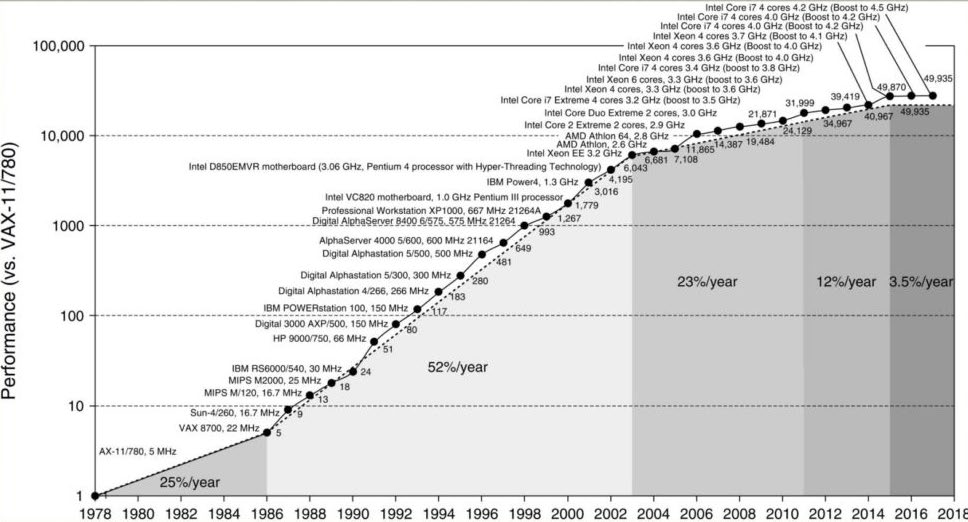
\includegraphics[width=.9\textwidth]{figure_parallel/moore2.png}
\end{subfigure}
\end{figure}

\subsection{Hardware parallelism}

How to avoid saturation?\\
Instruction level parallelism achieved significant performance advantages.But the performance are related to clock speed. Increasing in ILP is still possibile but the complexity of CPU is more than linear, diminishing return in efficiency.\\
\textbf{We need a next level in parallelism!}

\subsection{Flynn’s taxonomy}
Classification of computers architectures based on the number of data streams and instructions streams.
\begin{itemize}
    \item Single Instruction Single Data (SISD): Traditional sequential computing
    \item Singe Instruction Multiple Data (SIMD)
    \item Multiple Instructions Single Data (MISD)
    \item Multiple Instructions Multiple Data (MIMD)
\end{itemize}

\subsection{SISD: Single Instruction Single Data}
Only one instruction operates for
each time slot on one data (sequential processing).


\begin{figure}[ht]
\centering
\begin{subfigure}{.7\textwidth}
  \centering
  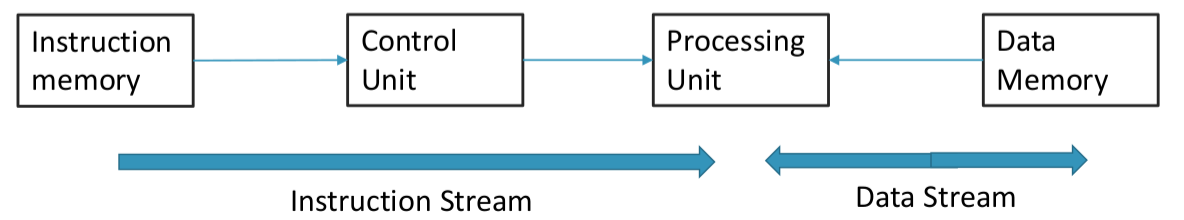
\includegraphics[width=.9\textwidth]{figure_parallel/sisd2.png}
\end{subfigure}%
\begin{subfigure}{.3\textwidth}
  \centering
  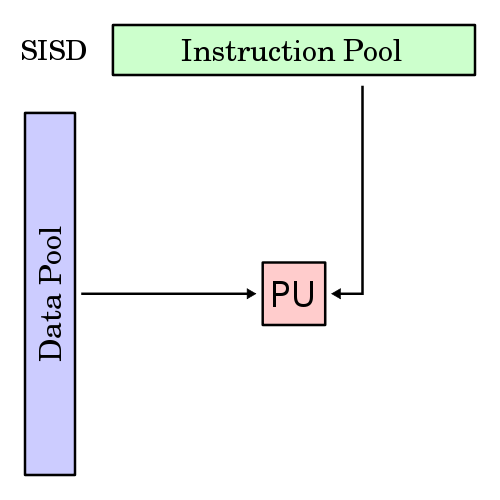
\includegraphics[width=.9\textwidth]{figure_parallel/SISD.png}
\end{subfigure}
\end{figure}

\subsection{SIMD: Single Instruction Multiple Data}

At one time one instruction operates on multiple data.

\begin{itemize}
    \item Very similar to vector processors (although in the vector architecture the parallelism is obtained with a pipeline, while in SIMD the operations are really parallel on vector’s element.)
    \item Array processors
    \item Most modern processors contain one or more SIMD sections
\end{itemize}

\begin{figure}[ht]
\centering
\begin{subfigure}{.7\textwidth}
  \centering
  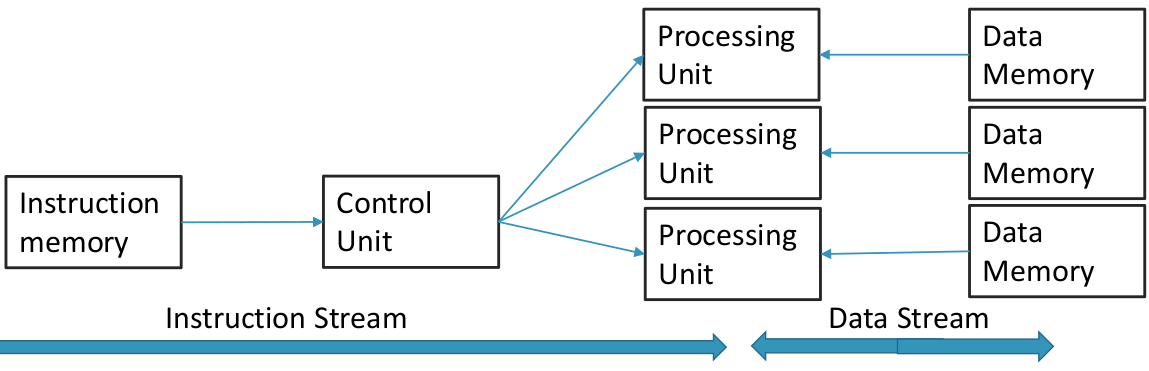
\includegraphics[width=.9\textwidth]{figure_parallel/simd.png}
\end{subfigure}%
\begin{subfigure}{.3\textwidth}
  \centering
  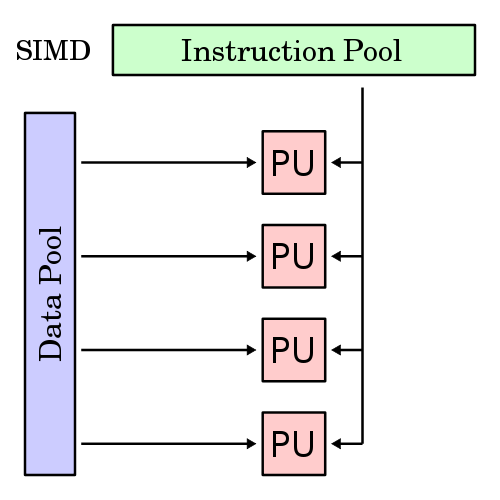
\includegraphics[width=.9\textwidth]{figure_parallel/simd2.png}
\end{subfigure}
\end{figure}

\subsection{MIMD: Multiple Instruction Multiple Data}

Multiple instructions streams operate on multiple data stream.
\begin{itemize}
    \item Most of supercomputers are organized as MIMD architecture
    \item Multi-core superscalar, multi-processors and distributed systems
\end{itemize}

\begin{figure}[ht]
\centering
\begin{subfigure}{.7\textwidth}
  \centering
  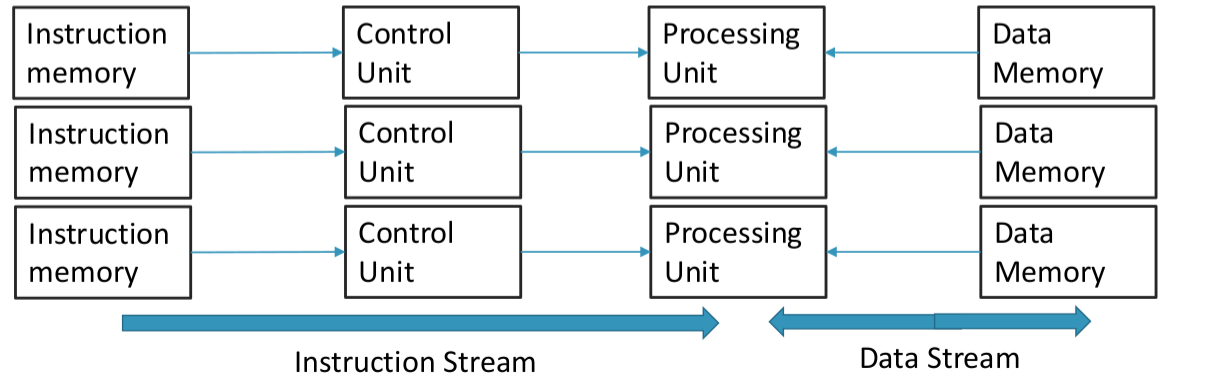
\includegraphics[width=.9\textwidth]{figure_parallel/mimd.png}
\end{subfigure}%
\begin{subfigure}{.3\textwidth}
  \centering
  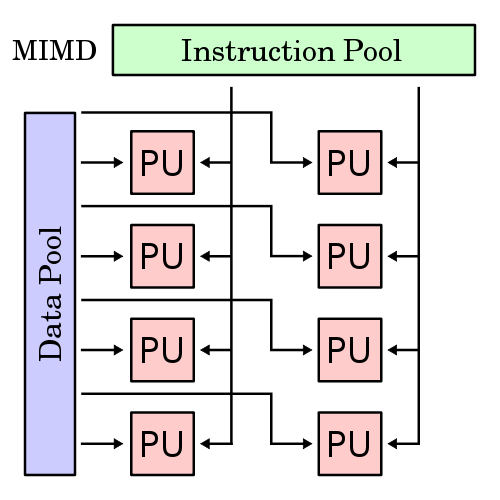
\includegraphics[width=.9\textwidth]{figure_parallel/mimd2.png}
\end{subfigure}
\end{figure}

\subsection{MISD: Multiple Instruction Single Data}
Not commonly seen. Sometime the systolic array is seen as MISD.\\
Usually is an architecture used for fault tollerance and not for computing.


\begin{figure}[ht]
\centering
\begin{subfigure}{.7\textwidth}
  \centering
  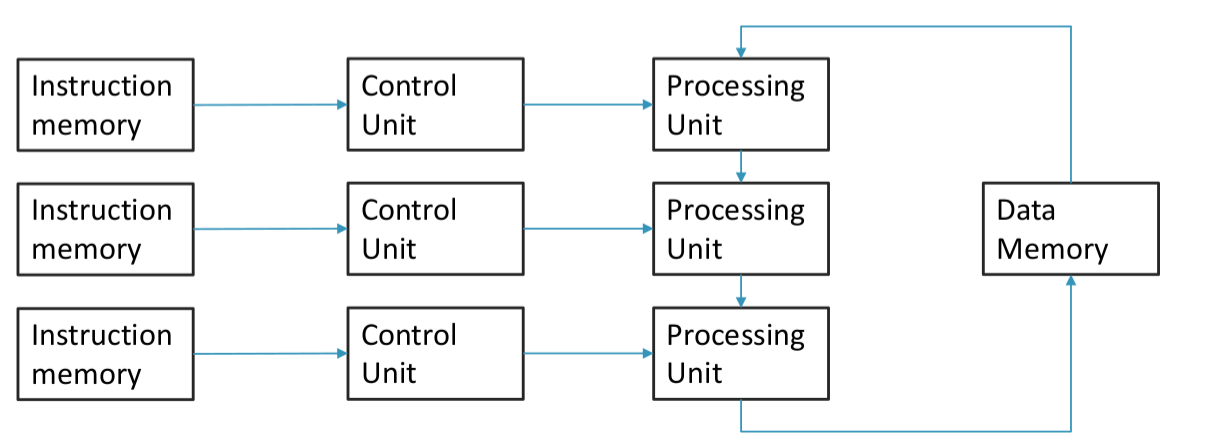
\includegraphics[width=.9\textwidth]{figure_parallel/misd.png}
\end{subfigure}%
\begin{subfigure}{.3\textwidth}
  \centering
  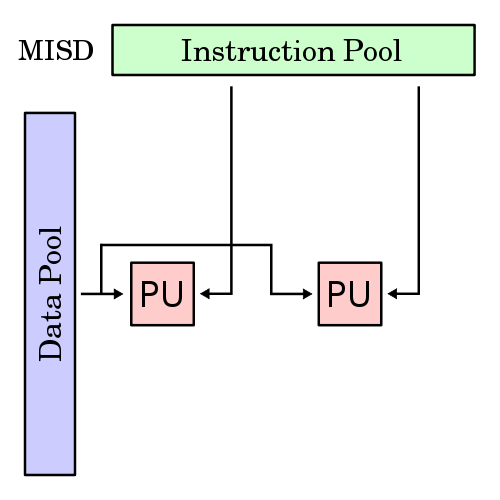
\includegraphics[width=.9\textwidth]{figure_parallel/misd2.png}
\end{subfigure}
\end{figure}

\subsection{Logic partitioning and decomposition}

\begin{wrapfigure}{r}{0.4\textwidth}
  \begin{center}
    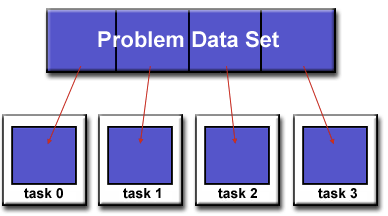
\includegraphics[width=0.35\textwidth]{figure_parallel/decomposition1.png}
    \vspace{5mm}
    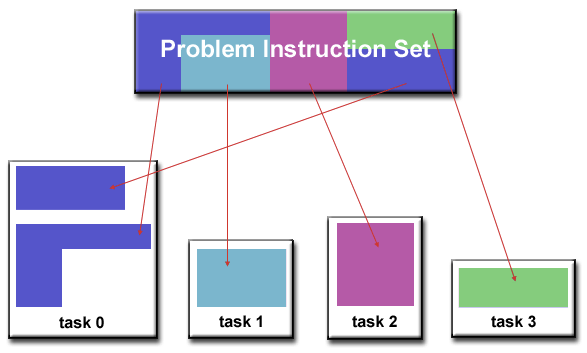
\includegraphics[width=0.35\textwidth]{figure_parallel/decomposition2.png}
  \end{center}
\end{wrapfigure}


The choice of the architecture depends on the problem.
\begin{itemize}
    \item Domain decomposition
    \begin{itemize}
        \item Single program, multiple data
        \item decomposition based on Input domain, output domain, both
    \end{itemize}
    \item Functional decomposition
        \begin{itemize}
        \item Multiple programs, multiple data
        \item Independent tasks
        \item Pipeling
    \end{itemize}
\end{itemize}

Ad esempio, se devo fare il prodotto tra matrici, divido le matrici in blocchi e faccio il prodotto.

\subsection{Multiprocessor Execution Model}
A specific architecture is suitable for a specific problem, but all needs «multiprocessors». Examples:
\begin{itemize}
    \item Each processor has its own PC and executes an independent stream of instructions (MIMD)
    \item Different processors can access the same memory space
    \item Processors can communicate via shared memory by storing/loading to/from common locations
\end{itemize}

\noindent
Two ways to use a multiprocessor:

\begin{itemize}
    \item Deliver high throughput for independent jobs via job-level parallelism
    \item Improve the run time of a single program that has been specially designed to run on a multiprocessor - a parallel-processing program
\end{itemize}


\subsection{Sequential processing}

Only one “thread” of execution:\\
-One step follows another in sequence\\
-One processor is all that is needed to run the algorithm\\

\textbf{Thread definition:} It is the smallest of a program that can be managed independently by a scheduler (typically in the operating system).\\

\noindent
- A thread is a component of a process\\
- Multiple threads can exist within one process\\
- Systems with a single processor generally implement multithreading by time slicing (software threads)


\begin{figure}[ht]
    \centering
    
\includegraphics[width=0.7\textwidth]{figure_parallel/ant_sequential.png}\end{figure}
\FloatBarrier

\subsection{Concurrent Processing}

A system in which:\\
-Multiple tasks can be executed at the same time\\
-The tasks may be duplicates of each other, or distinct tasks\\
-The overall time to perform the series of tasks is reduced\\

\noindent
\textbf{Advantages:}\\
-Concurrent processes can reduce duplication.\\
-The overall runtime of the algorithm can be significantly reduced.\\
-More real-world problems can be solved than with sequential algorithms alone.\\

\noindent
\textbf{Disadvantages}\\
-Runtime is not always reduced, so careful planning is require\\
-Concurrent algorithms can be more complex than sequential algorithms\\
-Shared data can be corrupted\\
-Communication between tasks is needed\\


\begin{figure}[ht]
    \centering
    
\includegraphics[width=0.7\textwidth]{figure_parallel/ant_concurrent.png}\end{figure}
\FloatBarrier

\newpage

\begin{wrapfigure}{r}{0.4\textwidth}
  \begin{center}
    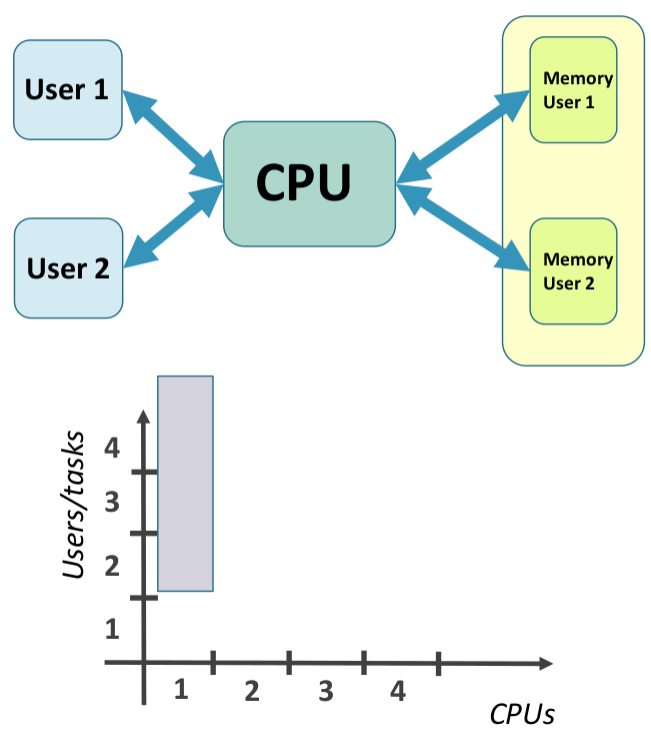
\includegraphics[width=0.38\textwidth]{figure_parallel/multiprogramming.png}
  \end{center}
  \caption{Multiprogramming \label{multiprog}}
\begin{center}
    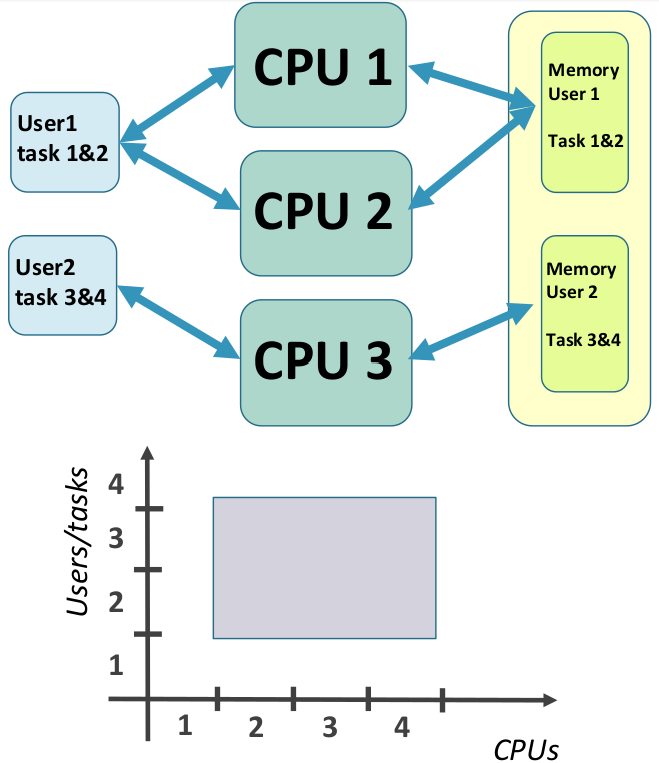
\includegraphics[width=0.38\textwidth]{figure_parallel/multiprocessing.png}
  \end{center}
  \caption{Multiprocessing \label{multiproc}}
\end{wrapfigure}

\subsection{Types of concurrent processing:}
-Multiprogramming\\
-Multiprocessing\\
-Multitasking\\
-Distributed Systems\\

\subsection{Multiprogramming}





-Share a single CPU among many users or tasks.\\
-May have a time-shared algorithm or a priority algorithm for determining which task to run next\\
-Gives the illusion of simultaneous processing through rapid swapping of tasks (interleaving).

\subsection{Multiprocessing}

-Executes multiple tasks at the same time\\
-Uses multiple processors to accomplish the tasks\\
-Each processor may also timeshare among several tasks\\
-Has a shared memory that is
used by all the tasks

\subsection{Multitasking}

-A single user can have
multiple tasks running at the
same time.\\
-Can be done with one or
more processors.\\
-Used to be rare and for only
expensive multiprocessing
systems, but now most
modern operating systems
can do it.\\

\subsection{Distributed systems}

-Multiple computers
working together with no
central program “in
charge.”\\
-No bottlenecks from
sharing processors\\
-No central point of failure\\
-Complexity\\
-Communication overhead\\
-Distributed control\\


\begin{figure}[ht]
\centering
\begin{subfigure}{.5\textwidth}
  \centering
  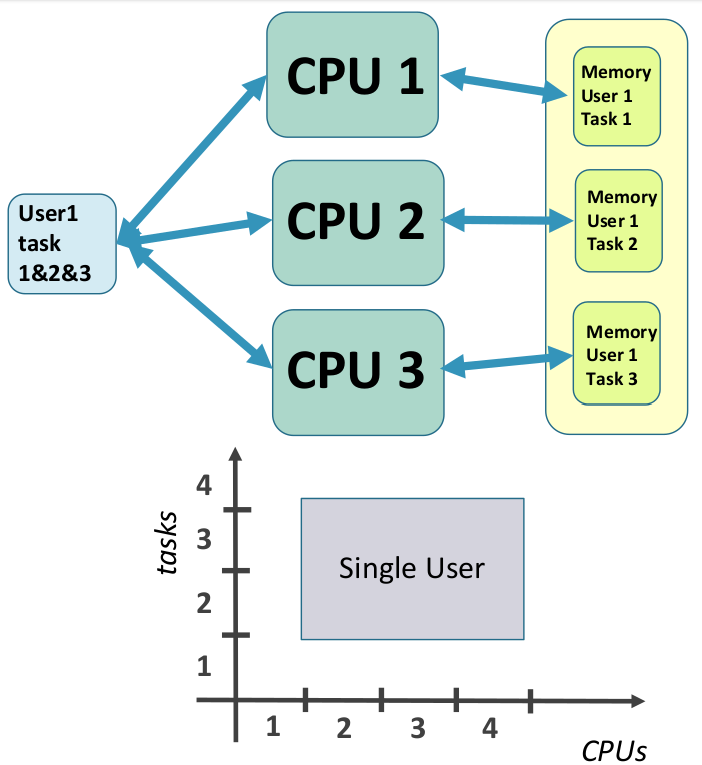
\includegraphics[width=.7\textwidth]{figure_parallel/multitasking.png}
  \caption{Multitasking}
\end{subfigure}%
\begin{subfigure}{.5\textwidth}
  \centering
  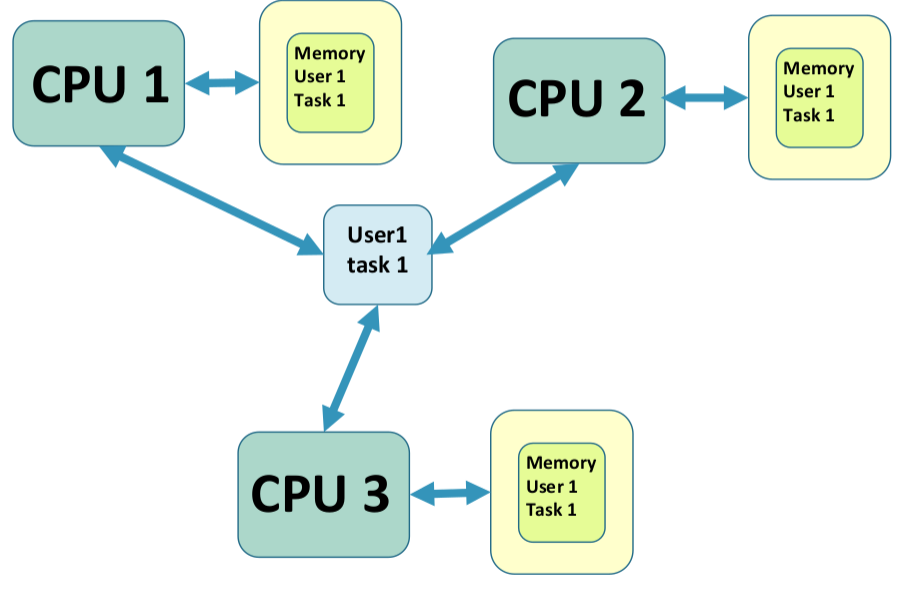
\includegraphics[width=.9\textwidth]{figure_parallel/distributed_system.png}
  \caption{Distributed Systems}
\end{subfigure}
\end{figure}

\newpage
\clearpage

\subsection{Parallelism vs Concurrency}

\textbf{Concurrency} is the execution of multiple tasks at the same time, regardless
of the number of processors.\\
\textbf{Parallelism} is the execution on multiple processors on the same task:
-Breaking the task into meaningful pieces\\
-Doing the work on many processors\\
-Coordinating and putting the pieces back together.


\begin{figure}[ht]
    \centering
    
\includegraphics[width=0.7\textwidth]{figure_parallel/ant_parallelism.png}\end{figure}
\FloatBarrier


\subsection{Parallelization}

\begin{wrapfigure}{r}{0.4\textwidth}
  \begin{center}
    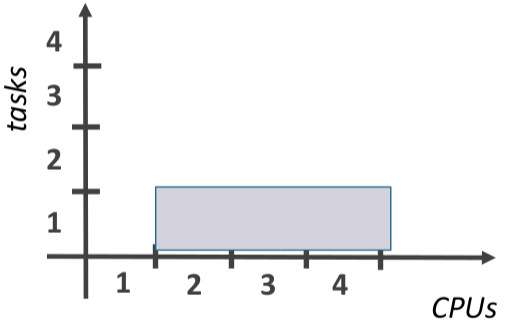
\includegraphics[width=0.38\textwidth]{figure_parallel/parallelization.png}
  \end{center}
\end{wrapfigure}

For a wide class of algorithms parallelization is the most powerfull way to decrease execution time (not complexity).\\
-Example: a problem with O(NlogN) complexity (for
instance Quicksort) on logN processors will take the
time needed by O(N) algorithms\\
-Example: a problem with O(N$^2$) complexity (for
instance binary search) on N processors will take the
time needed by O(N) algorithms\\

\noindent
\textbf{Parallelization is not free}. Processors must be controlled and coordinated. We need a way to govern which processor does what
work; this involves extra work.\\

Often the program must be written in a special programming language for parallel systems.
Often, a parallelized program for one machine (with, say, 2K processors) is not optimal on other machines (with, say, 2L processors).


\subsection{Speedup and Efficiency}

\begin{wrapfigure}{r}{0.4\textwidth}
  \begin{center}
    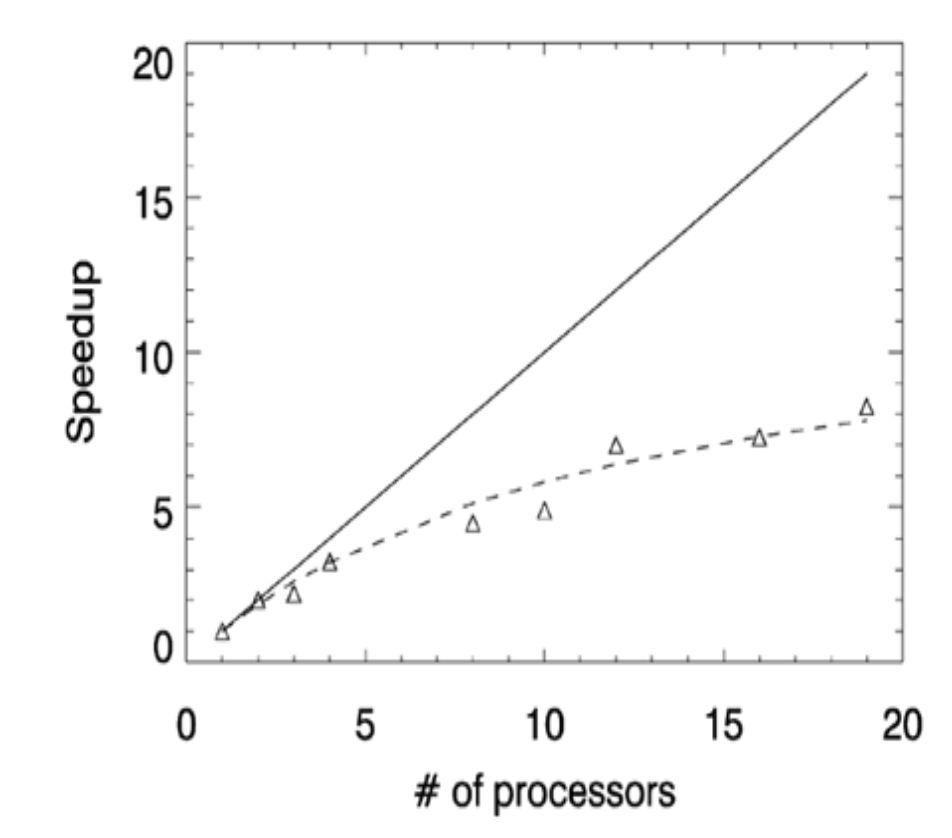
\includegraphics[width=0.38\textwidth]{figure_parallel/speedup.png}
  \end{center}
\end{wrapfigure}

How much gain can we get from
parallelizing an algorithm?\\
Let’s define the «speedup» as (where
n is the number of processors):

\begin{equation*}
    S_n = T_{serial}/T_{parallel}(n)
\end{equation*}

For a perfect parallel algorithm $S_n = n$. That's pratically impossible, even if for very specific cases could be also $S_n > n$ (superlinear case).\\

The efficiency is defined as:
\begin{equation}
    E = S_n/n
\end{equation}
It is a measure of how well our algorithm is using the processors.

\subsection{Cost and Scalability}

\textbf{Cost}: the number of CPU required
\begin{equation*}
    c = n T_p(n) = \dfrac{T_1}{E}
\end{equation*}

\textbf{Scalability}: capability to remain efficient with the increasing of the number of processors.

\subsection{Amdhal’s law (1967)}

\begin{wrapfigure}{r}{0.5\textwidth}
  \begin{center}
    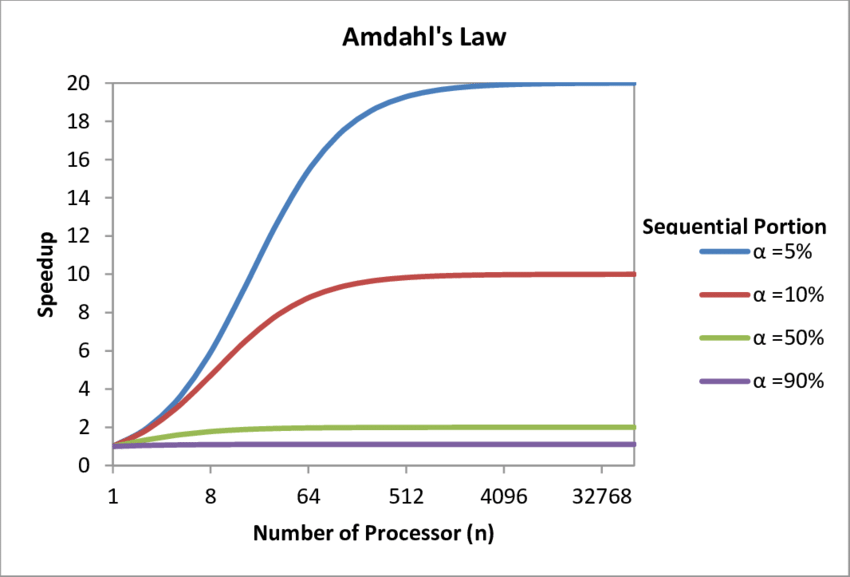
\includegraphics[width=0.48\textwidth]{figure_parallel/amdahl.png}
  \end{center}
\end{wrapfigure}

If only one part ($P_K$) of the code can be improved, the maximum improvement is given by:

\begin{equation*}
    1/\sum\dfrac{P_K}{S_K}
\end{equation*}

Where k is the part of the code and $S_k$ is the speedup of the part-k.\\

In the case of parallel programming:

\begin{equation*}
    S_n = \dfrac{n}{nF + (1-F)}
\end{equation*}

if $n \longrightarrow \infty$ the speedup is $S_n = 1/F$\\
For instance if the fraction of serial code is 10\% (F=0.10) the maximum speedup is «only» 10 (regardless the number of processors).\\
Apparently the parallelism is usefull only for «embarassingly parallel» problems, with a small number of processors.



\subsection{Overhead of parallelization}

\textbf{Load balancing}\\
In case of several tasks in parallel the execution time of each task must be similar. Otherwise the total time is dominated by the slower task.\\
Some processor could be inefficently IDLE. It’s not easy to design a priori a good load balancing.\\

\textbf{Synchronization}\\
If the tasks use the same memory (shared memory) to exchange data a logic of lock-unlock must be designed. This involves a waste of time.\\

\textbf{Comunication latency}\\
If data must be moved between processors the overhead due to data transmission can be really relevant.

\subsection{Limits of Amdhal’s law}
Apparently the Amdahl’s law puts important limits to the advantages of parallel computing. But there are importants caveat to this law:

-Amdahl assumes that the best solution is always the best serial
algorithm. Often some problem must be solved in parallel\\
-Some architectural design can help parallel processing (for instance
the caching)\\
-Amdahl assumes that the dimension of the problem is always the
same with the increasing of the number of processors. But more
processors often means that wider problem can be addressed.

\subsection{Gustafson’s law (1988)}
Let’s assume s is the time of the serial part (and p is the time parallel part).\\
Let’s assume that the problem grows with the number of processor (N) and that the serial part remains always the same.\\
Under these assumptions the speedup is given by:

\begin{equation*}
    s_n = N + (1-N)s
\end{equation*}

The speedup is linear with N.


\begin{figure}[ht]
\centering
\begin{subfigure}{.5\textwidth}
  \centering
  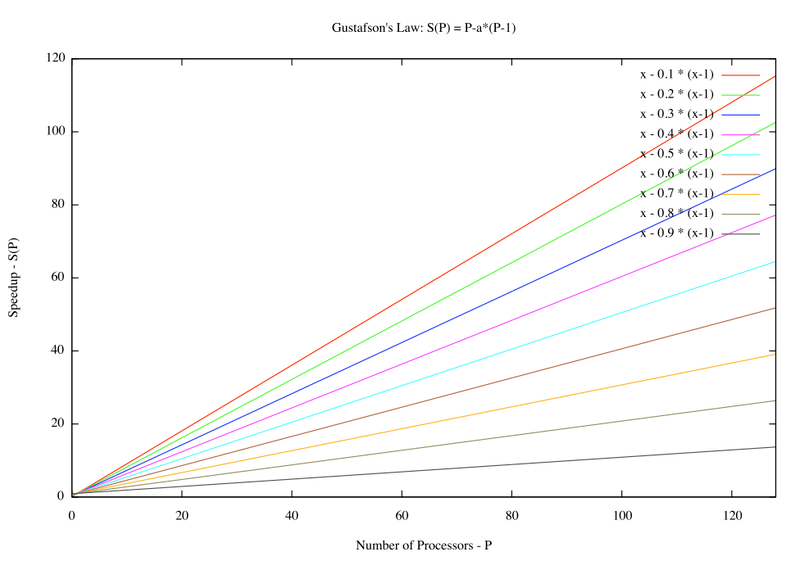
\includegraphics[width=.9\textwidth]{figure_parallel/gustafson1.png}
\end{subfigure}%
\begin{subfigure}{.5\textwidth}
  \centering
  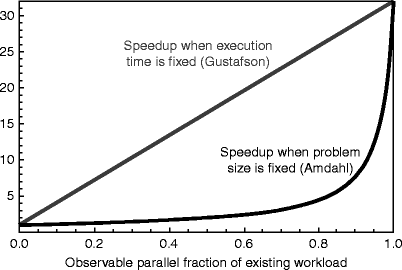
\includegraphics[width=.9\textwidth]{figure_parallel/gustafson2.png}
\end{subfigure}
\end{figure}

\vfill

\begin{tcolorbox}[width=\textwidth,colback={white},title={Recap: },colbacktitle=cyan,coltitle=black]

Standard processors are designed for “sequential” programming\\

-Several “tricks” are applied at instruction level to better exploit the Von Neuman structure (Vector processors, superscalars, pipeline, ...)\\

-Starting from about 2005 the performances serial processors start to show saturation (Moore’s law, Denard’s scaling)\\

-To overcome these limitations it is necessary to rethink the way of programming (Concurrency \& Parallelism)\\

-The idea: divide the problem in sub-problems to be addressed simultaneously (different architectures for parallelism: Flynn’s taxonomy)
\end{tcolorbox}


\newpage

\section{Multithreading and  multiprocessing in Python}

\subsection{Threads and processes}
Threads and processes are the way to use concurrency in python.\\ Python implements a very simple thread-safe mechanism: Global Interpreter Lock (GIL). In order to prevent conflicts only one statement in one thread is executed at a time (single-threading).\\


\begin{figure}[ht]
    \centering
    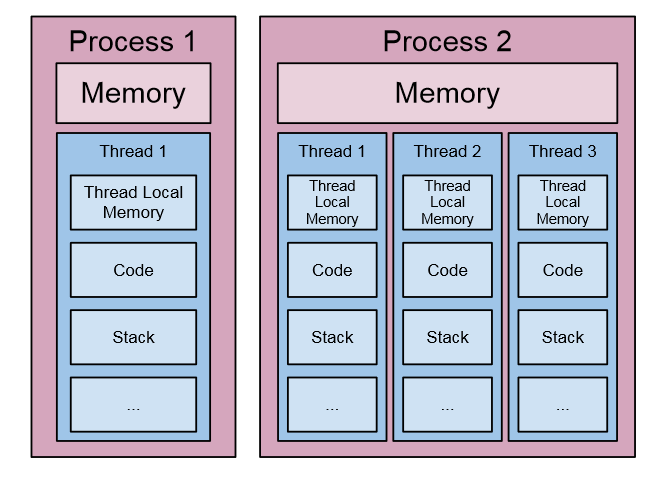
\includegraphics[width=0.6\textwidth]{figure_parallel/Thread_and_processes.png}\end{figure}
\FloatBarrier

\subsection{The Global Interpreter Lock (GIL)}

The Global Interpreter Lock refers to the fact that the Python interpreter is not thread safe. There is a global lock that the current thread holds to safely access Python objects. Because only one thread can acquire Python Objects/C API, the interpreter regularly releases and reacquires the lock every 100 bytecode of instructions. The frequency at which the interpreter checks for thread switching is controlled by the
\texttt{sys.setcheckinterval()} function. In addition, the lock is released and reacquired around potentially blocking I/O operations.\\
It is important to note that, because of the GIL, the CPU-bound applications won't be helped by threads. In Python, it is recommended to either use processes, or create a mixture of processes and threads. \\

\subsection{Processi e Thread}
Il processo è un'istanza del programma che abbiamo scritto. Ogni processo ha una memoria dedicata.\\
Quando due processi vengono lanciati, le due memorie non si parlano tra loro, sono completamente separate. Ogni processo ha una memoria chiusa.\\

All'interno di un singolo processo possiamo creare task differenti. Queste task possono essere viste come parti diverse del programma eseguite in modo seriale (ad es quando definiamo più funzioni che fanno compiti differenti per rendere più leggibile il programma).\\
Possiamo rendere questi task dei \textit{thread}: pezzi di codice che runna indipendentemente dagli altri.\\
C'è una memoria comune che è la memoria del processo. Poi ci sono thread diversi che runnano su risorse differenti (o sulla stessa risorsa) contemporaneamente.\\

Qualche volta è necessario che questi thread che stanno lavorando insieme, comunichino tra di loro. Magari vogliono leggere o scrivere qualcosa sulla memoria condivisa.Serve un meccanismo di comunicazione tra i vari thread. In che modo farli comunicare dipende da noi.\\


Il sistema operativo mette a disposizione due modi per mettere in comunicazione i thread, cercando di evitare possibili conflitti.
\textbf{Mutex}: è un sistema di locking: quando un thread vuole accedere a una parte di memoria o a una risorsa hardware, dice "questo lo sto usando io" e gli altri thread devono mettersi in coda fino a quando il lock non viene sganciato.\\
\textbf{Meccanismo dei Semafori}: si basa sul fatto che un thread comunichi agli altri thread cosa sta facendo. Nel caso del Mutex vince chi mette il lock e solo lui può toglierlo. Nel caso del semaforo c'è un meccanismo di priorità logica che permette a qualcun altro di prendere in mano la risorsa.\\

Python non permette di fare thread! Python è un linguaggio pensato per essere semplice, nel senso che impedisce di fare troppe cavolate.\\
Python è un linguaggio fortemente tipizzato. Non dichiaro mai le variabili, ma dopo che faccio \texttt{a = 1}, da quel punto la variabile è un intero e non posso cambiarlo, non posso successivamente scrivere \texttt{a = 1.5}.\\
\noindent
GIL = Global Interpreter Lock. Si possono definire i thread, ma fisicamente non vengono runnati insieme, bensì in modo seriale.
Allora perché farlo?\\
I thread sono utili quando è necessario fare I/O.\\
Se ho un thread che deve accedere a un file, python me lo permette.\\

Se voglio fare roba concorrenziale di \textbf{calcolo} contemporaneamente? Dobbiamo utilizzare i \textit{processi}: istanze di programmi.\\

Posso dire che tre funzioni all'interno di un programma vengano fatte in processi differenti, che effettivamente runneranno in parallelo. Questo ha lo svantaggio che i processi abbiano memorie differenti, quindi devo trovare un modo per farle comunicare.
Ho però il vantaggio di poter uccidere (kill) un singolo processo.\\

C'è un altro modo per fregare GIL, ovvero non usare python. Ad esempio quando usiamo alcune librerie, wrappate in python, ma scritte in C. E quelle librerie al loro interno usano i thread!\\

\textit{controllare di avere i moduli "multiprocessing" e "threading"}

\begin{tcolorbox}[width=\textwidth,colback={white},title={Process: pros and cons},colbacktitle=cyan,coltitle=black]
\textbf{pros:}\\
-A process is an instance of a program, managed by operating system (memory space allocated by the kernel).\\
-Two processes can executecode simultaneously in thesame python program\\
-Separated memory space\\
-Takes advantage of multiple cores and CPUs\\
-Child processes are killable\\
-Avoid GIL limitations\\
\textbf{cons:}\\
-Relatively high overhead\\
-Open and close processes takes more time\\
-Sharing information between processes is very slow\\
-Model not adaptable to parallelism
\end{tcolorbox}


\begin{tcolorbox}[width=\textwidth,colback={white},title={Threads: pros and cons},colbacktitle=green,coltitle=black]
\textbf{pros:}\\
-Processes produce threads (sub-processes) to handle sub-tasks (threads live inside the process and share the same memory space)\\

-Can use shared memory\\
-Threads communication\\
-Lightweight\\
-Very small overhead\\
-Great option for I/O bound application\\
\textbf{cons:}\\
-Subject to GIL (although there are workarounds)\\
-Not killable\\
-Potential of race condition \\
-Same memory space
\end{tcolorbox}

\subsection{When to use threads vs processes?}
\textbf{Processes} speed up Python operations that are CPU intensive because they benefit from multiple cores and avoid the GIL.\\
\textbf{Threads} are best for IO tasks or tasks involving external systems because threads can combine their work more efficiently. Processes need to pickle their results to combine them which takes time.\\

Threads provide no benefit in python for CPU intensive tasks because of the GIL.

\subsection{Things to be afraid of! (not only in python...)}

\textbf{Starvation}: a task is costantly denied necessary resource. The task can never finish (starves).\\
\textbf{Deadlock}: Usually a deadlock occurs when two or more tasks wait cyclically for each other.


\begin{figure}[ht]
    \centering
    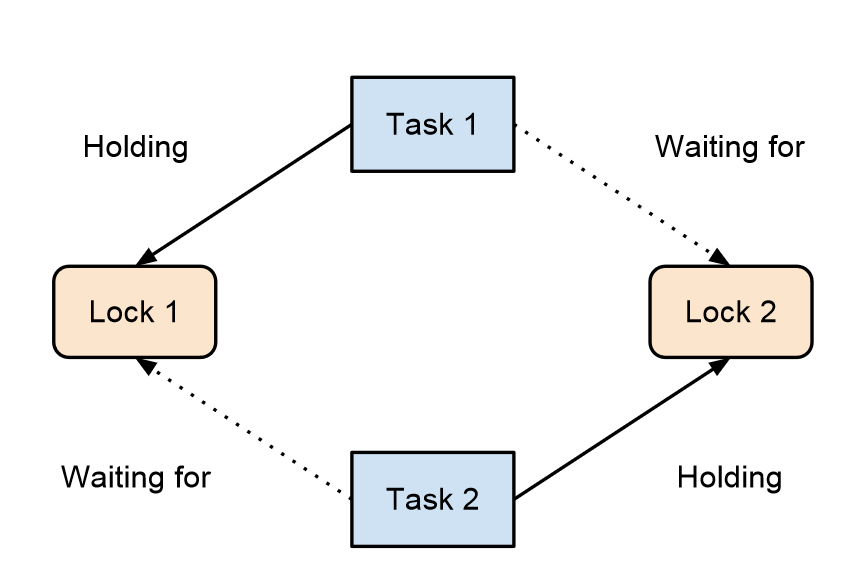
\includegraphics[width=0.5\textwidth]{figure_parallel/deadlock.png}\end{figure}
\FloatBarrier

\newpage
\section{\textit{Lun 24 ott - Lezione 10}}

\subsection{The multiprocessing module}
\subsubsection{HelloWorld}
Create a process
to run the function
f()

\inputminted{python}{python_parallel/HelloWorld.py}



Trasformeremo quello che fa la funzione in un processo.\\
Una volta definito il processo, lo dobbiamo fare partire usando il metodo \texttt{p.start}.
L'esecuzione di un thread può avvenire in modo sincrono e asincrono. Tipicamente avviene in modo asincrono: quando l'interprete trova \texttt{p.start} avvia il processo. Il processo parte; Il controllo del flusso va direttaente alla riga successiva, indipendentemente dl fatto che il processo sia terminato.
Questo succede a meno che non utilizziamo \texttt{p.join}. In tal caso il processo avviene in modo sincrono: finché non è finito il processo, si aspetta.

\subsubsection{FatherAndSons}
Generate a tree of processes

\inputminted{python}{python_parallel/FatherAndSons.py}


Ho un processo main in cui viene chiamata la funzione f0. Il main genera un processo, definito dalla funzione f1, nel quale viene chiamata f2.\\

\begin{figure}[ht]
    \centering
    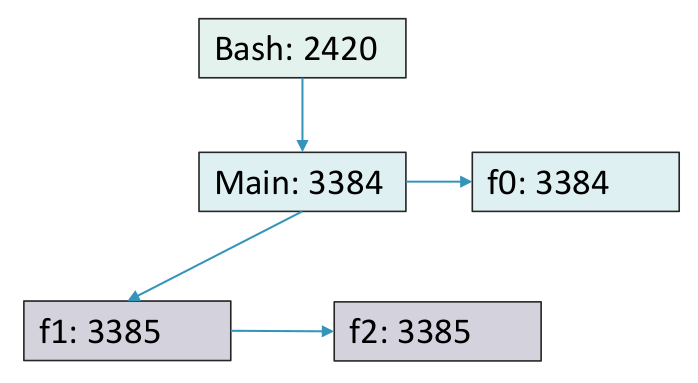
\includegraphics[width=0.5\textwidth]{figure_parallel/father_sons.png}\end{figure}
\FloatBarrier

Su linux, se sulla linea di comando scriviamo \texttt{ps}, mi dice quali processi sono in esecuzione.\\

\subsubsection{Use the Queue to get the result from multiple processes}

\inputminted{python}{python_parallel/FourProcesses.py}


La queue è una scatola in cui mettiamo dentro il risultato dei vari processi, per poi aprirla nel main.\\
\textbf{nota:} non possiamo assumere l'ordine delle cose che facciamo. Lo scheduler decide quando far partire i processi, che potrebbero finire in un ordine diverso da quello atteso.

\subsubsection{How to distribute work to
workers (aka cpu cores)}
Use the Pool class.\\
Try \texttt{Pool.map}\\
Try \texttt{Pool.map\_async}\\
See also \texttt{Pool.apply} e \texttt{Pool.apply\_async}


\begin{minted}{python}
def cube(x):
    print (str(os.getpid())+" "+str(os.getppid()))
    return x**3
#MAIN
if __name__=="__main__":
    pool = mp.Pool(processes=4)
    results = pool.map(cube,range(1,7))
    print(results)
\end{minted}

\begin{minted}{python}
#MAIN
if __name__=="__main__":
    pool = mp.Pool(processes=4)
    results = pool.map_async(cube,range(1,7))
    print(results.get())
\end{minted}

\textbf{nota} i processi avviati con pool.map sono di per sé sincroni (e partono subito), perciò non serve usare \texttt{join} (e \texttt{start}).\\

\subsubsection{Another example with \texttt{pool.map} and \texttt{pool.map\_async}}
Notice the time
measurement

\begin{minted}{python}
import multiprocessing as mp
import time
import os
def doingstuffs(x):
    print ("Process: "+str(x)+" "+str(os.getpid()))
    time.sleep(1)
if __name__=="__main__":
    start=time.time()
    pool = mp.Pool(processes=4)
    results = pool.map(doingstuffs,range(1,10))
    end=time.time()
    print("elapsed time: "+str(end-start))
\end{minted}

\begin{minted}{python}
results = pool.map_async(doingstuffs,range(1,10))
#…
print(results.get())
\end{minted}


\subsection{Communication between processes}

Un modo per (\textit{illuderci di}) passare informazione da un processo al'altro è utilizzare le variabili globali.

\inputminted{python}{python_parallel/communication1.py}



\begin{figure}[ht]
    \centering
    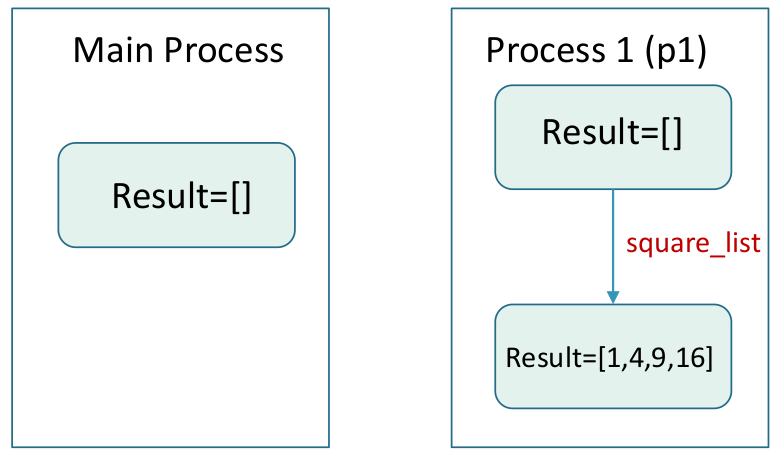
\includegraphics[width=0.45\textwidth]{figure_parallel/communication_global.png}\end{figure}
\FloatBarrier

Different memory spaces allocated for each process.
Try to print result in both processes.

\subsubsection{Comm. between processes: shared memory}

Normalmente abbiamo visto che le memorie sono separate. \'E possibile definire una zona di memoria (\textit{shared memory}) comune ad entrambi i processi.

\begin{figure}[ht]
    \centering
    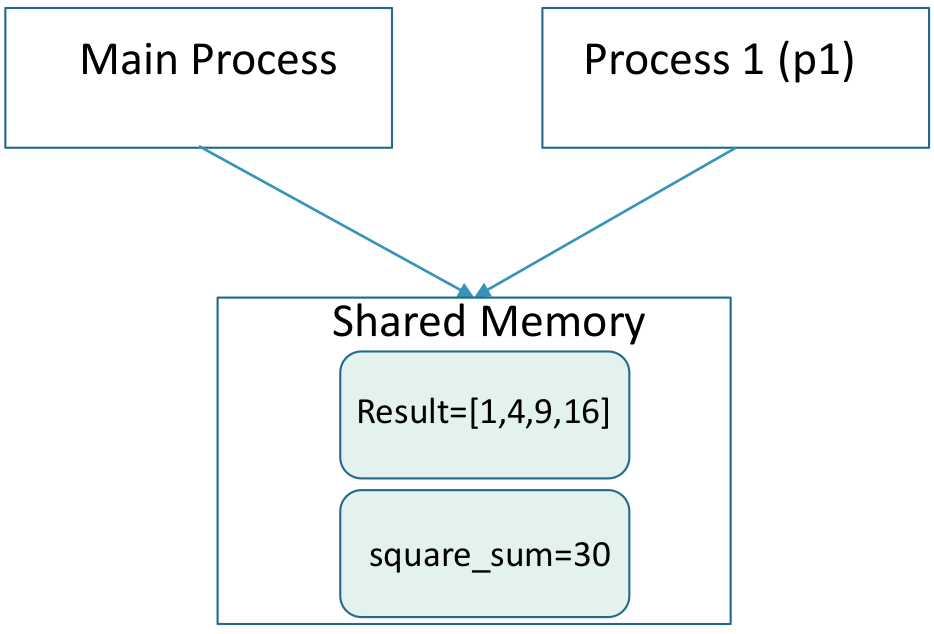
\includegraphics[width=0.45\textwidth]{figure_parallel/shared_memory.png}\end{figure}
\FloatBarrier

Shared memory:
multiprocessing module provides Array and Value objects to share data between processes.\\
\texttt{Array:} array allocated from shared
memory.\\
\texttt{Value:} object allocated from shared
memory.

\inputminted{python}{python_parallel/communication2.py}



Nella shared memory non posso mettere oggetti complicati come i dizionari.


\subsubsection{Comm. between processes: server process}


Server process : Whenever a python program
starts, a server process is also started. From
there on, whenever a new process is needed,
the parent process connects to the server and
requests it to fork a new process.
A server process can hold Python objects and allows
other processes to manipulate them.
multiprocessing module provides a Manager class
which controls a server process. Hence, managers
provide a way to create data which can be shared
between different processes.
Server process allows to share any type of object (dict,
lists,…). It is also possible to connect a server process
to the network

\inputminted{python}{python_parallel/communication3.py}

\begin{figure}[ht]
    \centering
    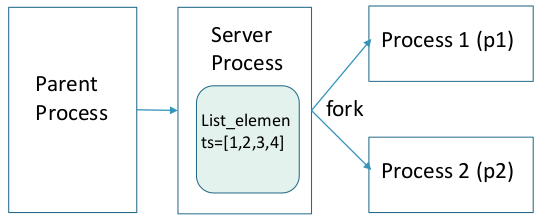
\includegraphics[width=0.55\textwidth]{figure_parallel/server_process.png}\end{figure}
\FloatBarrier

\subsubsection{Comm. between processes: queue}

\textbf{Queue :} A simple way to communicate between process with multiprocessing is to use a Queue to pass messages back and forth.\\
Any Python object can pass through a Queue.

\begin{figure}[ht]
    \centering
    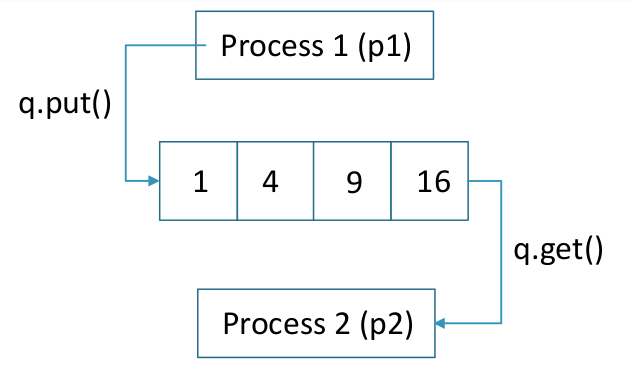
\includegraphics[width=0.45\textwidth]{figure_parallel/queue.png}\end{figure}
\FloatBarrier


\inputminted{python}{python_parallel/communication4.py}

\textbf{nota:} quando estraggo un elemento dalla coda, lo rimuovo da essa.


\subsubsection{Comm. between process: pipe}

In linea di principio, la coda permette di avere più \textit{endpoint}: non necessariamente entra da un lato ed esce da un altro. Invece la pipe è così: la dobbiamo immaginare proprio come un tubo.

\begin{figure}[ht]
    \centering
    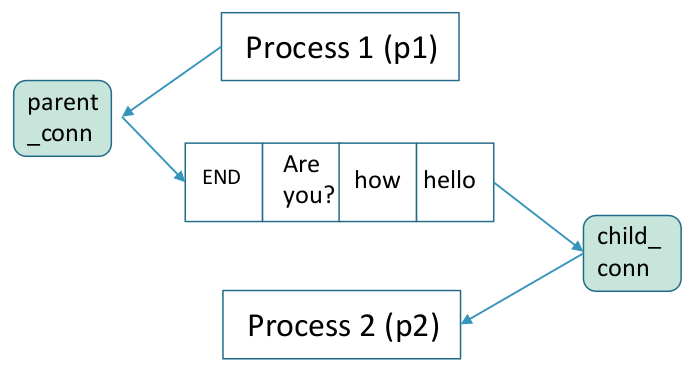
\includegraphics[width=0.5\textwidth]{figure_parallel/pipe.png}\end{figure}
\FloatBarrier

Se ho soltanto due processi: uno che scrive e uno che legge, allora è più conveniente usare le pipe perché sono più veloci.\\

\textbf{Pipes :} A pipe can have only two endpoints. Hence, it is preferred over queue when only two-way communication is required. Queue is slower (it’s built on top of pipe).\\

multiprocessing module provides \texttt{Pipe()} function which returns a pair of connection objects connected by a pipe.
The two connection objects returned by \texttt{Pipe()} represent the two ends of the pipe.
Each connection object has \texttt{send()} and \texttt{recv()} methods (among others).


\subsection{Synchronization between processes}

Process synchronization is defined as a mechanism which ensures that two or more concurrent processes do not simultaneously execute some particular program segment known as critical section. A race condition occurs when two or more processes can access shared data and they try to change it at the same time. As a result, the values of variables may be unpredictable and vary depending on the timings of context switches of the processes.

\inputminted{python}{python_parallel/synchro1.py}


Se permettiamo a due processi di scrivere contemporaneamente sulla stessa locazione di memoria succede un casino!

multiprocessing module provides a Lock class to deal with the race conditions. Lock is implemented using a Semaphore object provided by the Operating System. A semaphore is a synchronization object that controls access by multiple processes to a common resource in a parallel programming environment. It is simply a value in a designated place in operating system (or kernel) storage that each process can check and then change. Depending on the value that is found, the process can use the resource or will find that it is already in use and must wait for some period before trying again.

\inputminted{python}{python_parallel/synchro2.py}

Il lock si utilizza ogni volta che si vuole impedire che la stessa risorsa venga usata due volte.


\subsection{Threading}



A thread is an entity within a process that can be scheduled for execution. Also, it is the smallest unit of processing that can be performed in an OS (Operating System).\\
In simple words, a thread is a sequence of such instructions within a program that can be executed
independently of other code. For simplicity, you can
assume that a thread is simply a subset of a
process!
Multiple threads can exist within one process where:\\
-Each thread contains its own register set and local variables (stored in stack).\\
-All thread of a process share global variables (stored in heap) and the program code.

\begin{figure}[ht]
    \centering
    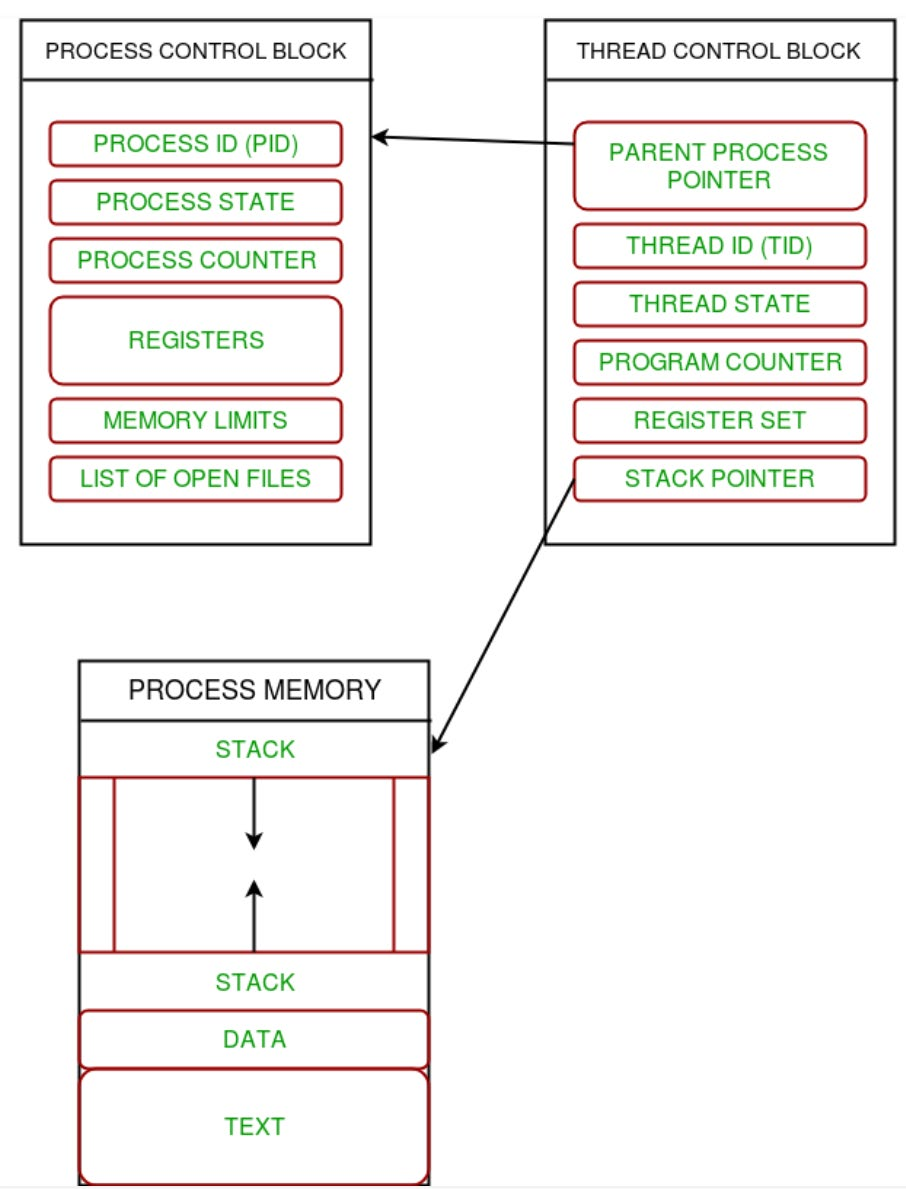
\includegraphics[width=0.45\textwidth]{figure_parallel/thread.png}\end{figure}
\FloatBarrier

\subsection{Threading module}



The threads aren’t different processes. Due to GIL the parallelism is only «Logic».

\inputminted{python}{python_parallel/thread1.py}


\subsection{Threads synchronization}

\inputminted{python}{python_parallel/thread2.py}
\inputminted{python}{python_parallel/thread2b.py}


\subsection{Comparison between Threads and Processes}

Write a code to factorize a list of numbers: the 300 odd numbers from 1000000000001 and 1000000000597.\\

Try to benchmark the time needed to factorize this list by using:\\
-Serial code\\
-2,4,8 Threads\\
-2,4,8 Processes\\
Produce a plot with the results


\begin{figure}[ht]
	\centering
	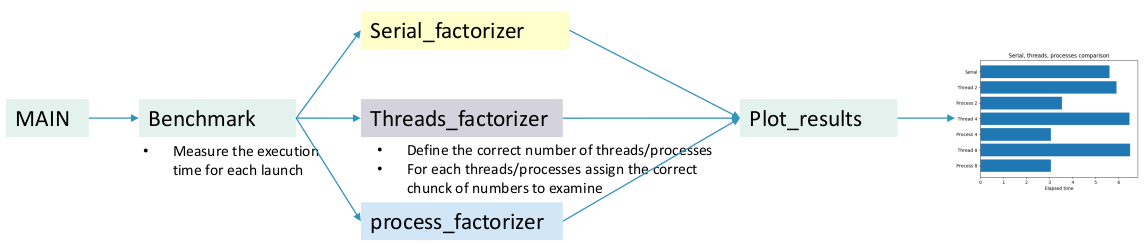
\includegraphics[width=1\textwidth]{figure_parallel/comparison_thread_processes.png}\end{figure}
\FloatBarrier


\inputminted{python}{python_parallel/final_example.py}


\begin{figure}[ht]
	\centering
	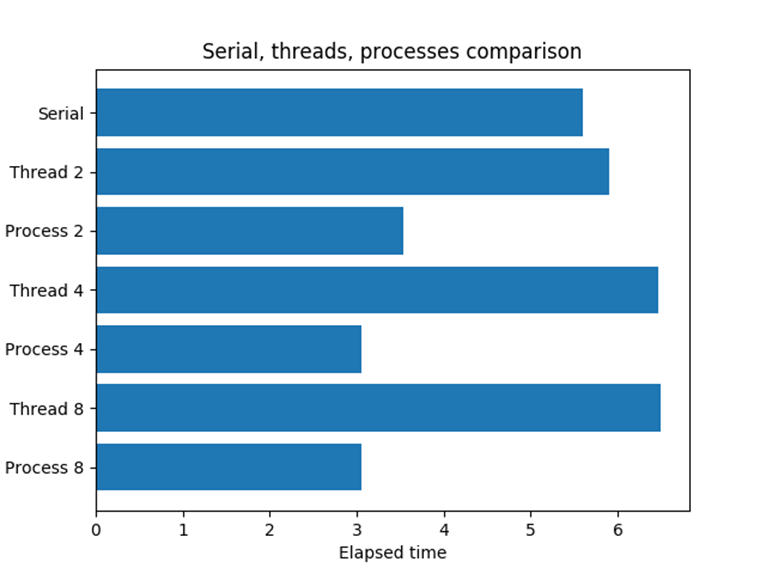
\includegraphics[width=0.5\textwidth]{figure_parallel/comparison_time.png}\end{figure}
\FloatBarrier

\subsection{Why should I use threads?}
GIL is bypassed in two cases:\\
-running programs in external C code (ex: numpy)\\
-in case of I/O operation: Python release the lock waiting for I/O\\

A tipical application is the use of the network. Writing to a disk, display an image to the screen, print on a printer,…



\begin{minted}{python}
import requests
import threading as thr
from time import perf_counter

buffer_size=1024
#define a function to manage the download
def download(url):
	response = requests.get(url, stream=True)
	filename = url.split("/")[-1]
	with open(filename,"wb") as f:
		for data in response.iter_content(buffer_size):
			f.write(data)

#MAIN
if __name__ == "__main__":
	urls= [
		"http://cds.cern.ch/record/2690508/files/201909-262_01.jpg",
		"http://cds.cern.ch/record/2274473/files/05-07-2017_Calorimeters.jpg",
		"http://cds.cern.ch/record/2274473/files/08-07-2017_Spectrometer_magnet.jpg",
		"http://cds.cern.ch/record/2127067/files/_MG_3944.jpg",
		"http://cds.cern.ch/record/2274473/files/08-07-2017_Electronics.jpg",
	]

	t = perf_counter()
#sequential download
	for url in urls:
		download(url)
	print("Time: "+str(perf_counter()-t))

\end{minted}


Versione parallela: faccio 5 thread che scaricano contemporaneamente 5 immagini:

\begin{minted}{python}

import threading as thr
import requests
import os
from time import perf_counter

buffer_size=1024

#define a function to manage the download
def download(url):
	response = requests.get(url, stream=True)
	filename = url.split("/")[-1]
	with open(filename,"wb") as f:
		for data in response.iter_content(buffer_size):
			f.write(data)
			
			
#MAIN
if __name__ == "__main__":
	urls= [
		"http://cds.cern.ch/record/2690508/files/201909-262_01.jpg",
		"http://cds.cern.ch/record/2274473/files/05-07-2017_Calorimeters.jpg",
		"http://cds.cern.ch/record/2274473/files/08-07-2017_Spectrometer_magnet.jpg",
		"http://cds.cern.ch/record/2127067/files/_MG_3944.jpg",
		"http://cds.cern.ch/record/2274473/files/08-07-2017_Electronics.jpg",
	]
	
#define 5 threads
	threads = [thr.Thread(target=download, args=(urls[x],)) for x in range(4)]

	t = perf_counter()
	
#start threads
	for thread in threads:
		thread.start()
		
#join threads
	for thread in threads:
		thread.join()
		
	print("Time: "+str(perf_counter()-t))
\end{minted}

Performaces depend on network speed. Overheads for thread start and lock release.


\subsection{Process vs Threads}

\begin{figure}[ht]
    \centering
    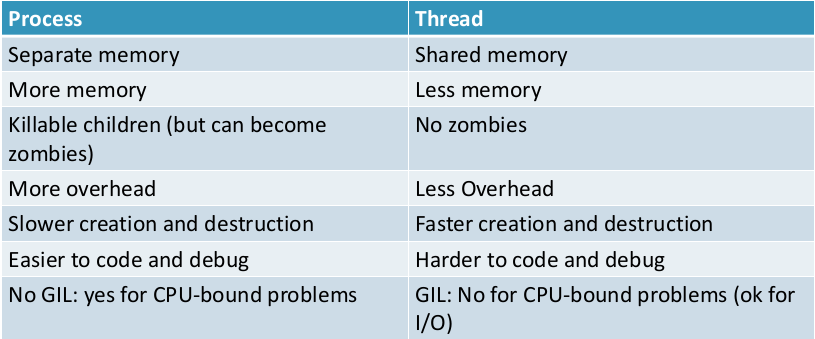
\includegraphics[width=0.7\textwidth]{figure_parallel/process_vs_thread.png}\end{figure}
\FloatBarrier



\newpage
\section{\textit{Gio 27 ottobre - Lezione 11}}
\section{Introduction to GPU computing (1)}

\subsubsection{Moore's Law}

Moore’s law: “The performance of microprocessors and the number of their transistors will double every 18 months”.\\
The increasing of performance is related to the clock.\\
Faster clock means higher dissipation $\rightarrow$ power wall

\begin{figure}[ht]
	\centering
	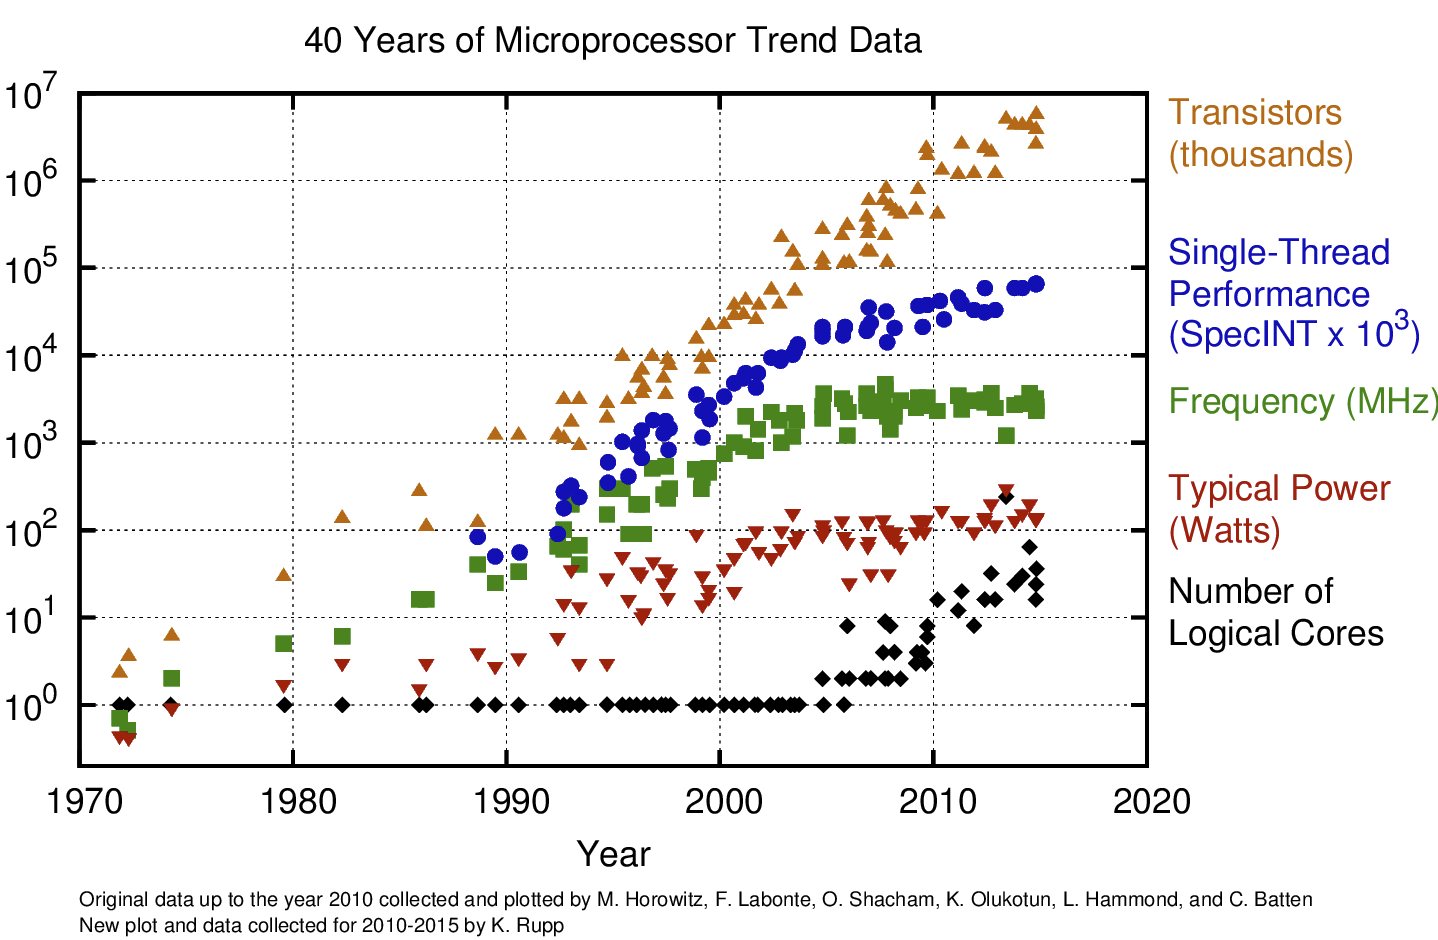
\includegraphics[width=0.5\textwidth]{figure_parallel/moore.png}\end{figure}
\FloatBarrier


\subsection{Parallel programming}

Parallel computing is no longer something for SuperComputers. All the processors nowadays are multicores.\\
The use of parallel architectures is mainly due to the physical constraints to
frequency scaling.

\begin{figure}[ht]
	\centering
	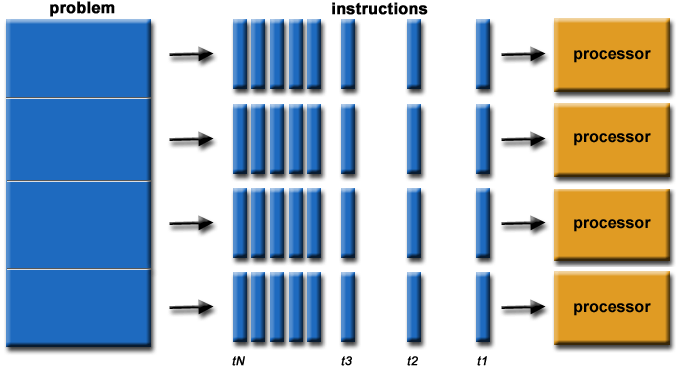
\includegraphics[width=0.5\textwidth]{figure_parallel/parallel_programming.png}\end{figure}
\FloatBarrier

\subsection{Limits of parallel programming}

Several problems can be split in
smaller problems to be solved
concurrently. In any case the maximum speedup is not linear , but it depends on the serial part of the code (Amdahls’s law)\\
The situation can improve if the
amount of parallelizable part
depends on the resources(Gustafson’s Law)

\begin{figure}[ht]
	\centering
	\includegraphics[width=0.5\textwidth]{figure_parallel/limits_parallel_programming.png}\end{figure}
\FloatBarrier

\begin{equation*}
	S_{latency} = \dfrac{1}{1-p+\frac{p}{s}}
\end{equation*}

\begin{equation*}
	S_{latency} = 1 - p + sp
\end{equation*}

\subsection{What are GPUs?}

The GPUs are processors dedicated to parallel programming for
graphical application.
Rendering, Image transformation, ray tracing, etc. are typical
application where parallelization can helps a lot.


\subsection{Standard GPU pipeline}

\begin{figure}[ht]
	\centering
	\includegraphics[width=1\textwidth]{figure_parallel/gpu_pipeline.png}\end{figure}
\FloatBarrier

Ogni triangolino è indipendente dall'altro. Possiamo agire contemporaneamente su questi triangolini in maniera parallela.

\subsection{Standard GPU requirements}

\textbf{Graphics pipeline}: huge amount of arithmetic on independent data:\\
-Transforming positions\\
-Generating pixel colors\\
-Applying material properties and light situation to every pixel\\
\textbf{Hardware needs}\\
-Access memory simultaneously and contiguously\\
-Bandwidth more important than latency\\
-Floating point and fixed-function logic\\

\subsection{What are the GPUs?}

The technical definition of a GPU is "a single-chip processor with integrated
transform, lighting, triangle setup/clipping, and rendering engines that is
capable of processing a minimum of 10 million polygons per second.“\\
The possibility to use the GPU for generic computing (GPGPU) has been
introduced by NVIDIA in 2007 (CUDA)\\
In 2008 OpenCL: consortium of different firms to introduce a multi-platform
language for manycores computing.

\subsection{Why the GPUs?}

-GPU is a way to cheat the Moore’s law\\
Implementano la possibilità di eseguire operazioni ad una velocità superiore a quella del clock.\\
-SIMD/SIMT parallel architecture\\
-The PC no longer get faster, just wider.\\
-Very high computing power for «vectorizable» problems\\
-Impressive derivative almost a factor of 2 in each generation\\
-Continuous development\\
-Easy to have a desktop PC with teraflops of computing power, with thousand of cores.\\
-Several applications in HPC, simulation, scientific computing…\\

Vogliamo imparare a sfruttare una tecnologia utilizzata sul mercato (che migliora ogni anno), per i nostri scopi di calcolo scientifico.\\

\subsection{A lot of cores...}

\begin{figure}[ht]
	\centering
	\includegraphics[width=0.5\textwidth]{figure_parallel/cores.png}\end{figure}
\FloatBarrier


\begin{figure}[ht]
	\centering
	\includegraphics[width=0.5\textwidth]{figure_parallel/cores2.png}\end{figure}
\FloatBarrier


\subsection{Metrics}

\textbf{FLOPS} (Floating Point operation per
second):\\
It is a measurement of the computing power of a processor. Theoretically is defined as:
\begin{equation*}
	FLOPS = clock * cores * Operation/cycle
\end{equation*}
%%%%
Actually this formula doesn’t take into account several things\\
The real extimation is made experimentally by using standard packages (LINPACK,
LAPACK)\\
The FLOPS is only a first indication of the computing power.\\
Other metrics has been invented to avoid the limitations of the FLOPS.\\

\textbf{SPECint and SPECf}\\
They are suites of 12 benchmarks of different type (for integer and floating point). The extimation is relative to a particular
machine.



\begin{figure}[ht]
\centering
\begin{subfigure}{.5\textwidth}
	\centering
	\includegraphics[width=.9\linewidth]{figure_parallel/metrics.png}
\end{subfigure}%
\begin{subfigure}{.5\textwidth}
	\centering
	\includegraphics[width=.9\linewidth]{figure_parallel/metrics2.png}
\end{subfigure}
\end{figure}
\FloatBarrier







\subsection{Computing power comparison}

\begin{figure}[ht]
	\centering
	\includegraphics[width=0.9\textwidth]{figure_parallel/computing_power_comparison.png}\end{figure}
\FloatBarrier

\subsection{CPU}

-\textbf{Multilevel and Large Caches}: Convert long latency memory access to -short latency cache latency.\\
-\textbf{Branch prediction:} To reduce latency in branching
-Instruction level parallelism (ILP)\\
-Powerful ALU: Reduced operation latency\\
-Memory management\\
-Large control part\\

\begin{figure}[ht]
	\centering
	\includegraphics[width=0.38\textwidth]{figure_parallel/CPU.png}
	\caption{CPU: latency oriented design}
\end{figure}
\FloatBarrier

\subsection{GPU}

-SIMT/SIMD (Single instruction Multiple Thread/Data) architecture\\
-SMX (Streaming Multi Processors) to execute kernels\\
-Thread level parallelism: Massive threading to hide the latency\\
-Limited caching: To boost memory throughput\\
-Limited control\\
-No branch prediction, but branch predication

\begin{figure}[ht]
	\centering
	\includegraphics[width=0.36\textwidth]{figure_parallel/GPU.png}
	\caption{GPU: throughput oriented design}
\end{figure}
\FloatBarrier

\subsection{CPU vs GPU}

\begin{figure}[ht]
	\centering
	\includegraphics[width=1\textwidth]{figure_parallel/cpu_vs_gpu.png}
\end{figure}
\FloatBarrier


\begin{figure}[ht]
	\centering
	\includegraphics[width=0.8\textwidth]{figure_parallel/cpu_vs_gpu_table.png}
\end{figure}
\FloatBarrier

\subsection{SIMT}


\begin{wrapfigure}{r}{0.45\textwidth}
	\begin{center}
		\includegraphics[width=0.43\textwidth]{figure_parallel/simt.png}
	\end{center}
\end{wrapfigure}

Consideriamo un processore da 4000 core. La struttura SIMD prevederebbe che tutti i core facciano la stessa cosa nello stesso momento (ad es sommare due vettori di 4000 elementi).



\begin{itemize}
	\item Standard CPU : Scalar processors
	\item SIMD CPU: vector processors
	\item Simultaneous threads in multicore processors
	\item SIMT (Single Instruction Multiple	Threads)
	\begin{itemize}
		\item CPU core ~ GPU multiprocessor (SMX)
		\item Working unit: a set of threads (32, a warp)
		\item Fast switching of threads
	\end{itemize}
\end{itemize}

\subsection{CPU core vs GPU SMX}

\begin{figure}[ht]
	\centering
	\includegraphics[width=1\textwidth]{figure_parallel/core_vs_smx.png}
\end{figure}
\FloatBarrier


The latency in a SMX is hidden thanks to very deep pipelines.\\
The multithreading in a single CPU core is based on context switching.\\



\subsection{GPU+CPU}

\begin{wrapfigure}{r}{0.5\textwidth}
	\begin{center}
		\includegraphics[width=0.3\textwidth]{figure_parallel/GPU_CPU.png}
	\end{center}
\end{wrapfigure}

The winning application uses both CPU and GPU:

\begin{itemize}
	\item CPUs for sequential parts
	\begin{itemize}
		\item can be 10X faster than GPU for sequential code
	\end{itemize}
	\item GPUs for parallel part where throughput wins
	\begin{itemize}
		\item can be 100X faster than CPU for parallel code
	\end{itemize}
	\item The Host-Device connection is done with PCIe-gen3 (16 GB/s) or NVLINK (80 GB/s)
	\begin{itemize}
		\item Relatively slow
		\item Do as little as possible
	\end{itemize}
	\item The bandwidth between GPU and video memory is HBM2 (720 GB/s in P100, 900 GB/s in V100)
\end{itemize}


\vfill

\begin{tcolorbox}[width=\textwidth,colback={white},title={Summary: },colbacktitle=cyan,coltitle=black]
	\begin{itemize}
		\item Superscalars, Pipelining and Vectorialization are methods to exploit some «parallelism» at the instruction and data level: ILP
		\begin{itemize}
			\item Probably OOO (Out-of-order) execution should be included in this category
		\end{itemize}
		\item The possible improvement thanks to ILP depends on problem and data structures
		\begin{itemize}
			\item 1x-10x for Superscalars and Pipeline
			\item 2x,4x,8x,16x for the vectorialization
		\end{itemize}
		\item These methods show «saturation» because they are limited by the CPU resources available
		\begin{itemize}
			\item Pentium 4: 30 pipeline stages (nowadays 10-15 maximum)
			\item ARM A57 (Apple A7/A8): 9 ports/6 instructions superscalar
			\item Intel Tiger Lake: vector of 512 bits for a subset of AVX512 instructions
		\end{itemize}
	\end{itemize}  
	… the point is: can CPU resources grow indefinitely?
\end{tcolorbox}

\newpage
\clearpage

\section{Introduction to GPU computing (2)}
\subsection{CUDA model}


\begin{figure}[ht]
	\centering
	\includegraphics[width=0.4\textwidth]{figure_parallel/cuda.png}
\end{figure}
\FloatBarrier

CUDA is a set of C/C++ extensions to enable the GPGPU computing on
NVIDIA GPUs. Dedicated APIs allow to control almost all the functions of the graphics processor.\\
Three steps:
\begin{enumerate}
	\item copy data from Host to Device
	\item copy Kernel and execute
	\item copy back results
\end{enumerate}

\subsection{Grid, blocks and threads}

The computing resources are logically (and physically) grouped in a flexible parallel model of computation:\\
\begin{itemize}
	\item 1D,2D and 3D grid
	\item With 1D, 2D and 3D blocks
	\item With 1D, 2D and 3D threads
\end{itemize}

Only threads can communicate and synchronize in a block.\\
Threads in different blocks do not interact, threads in same block execute same instruction at the same time.\\
The “shape” of the system is decided at kernel launch time.

\begin{figure}[ht]
	\centering
	\includegraphics[width=0.55\textwidth]{figure_parallel/gbt.png}
\end{figure}
\FloatBarrier

\subsection{GPU structure}
I singoli thread runnano sui core.
I thread sono raggruppate in blocchi. Un blocco è implementato da un multiprocessore.

\begin{figure}[ht]
	\centering
	\includegraphics[width=0.7\textwidth]{figure_parallel/gpu_structure.png}
\end{figure}
\FloatBarrier

\subsection{Multiprocessor}
Anche se il numero di core è più piccolo del numero di thread, continua a poterli runnare, perché lo scheduler si prende il compito di fare eseguire i vari compiti in maniera parallela.

\begin{figure}[ht]
	\centering
	\includegraphics[width=0.5\textwidth]{figure_parallel/multiprocessor.png}
\end{figure}
\FloatBarrier

\subsection{Memory}

The memory hierarchy is fundamental in GPU programming.
Most of the memory managing and data locality is left to the user.\\
\begin{itemize}
	\item Unified Address Space
	\item Global Memory
	\begin{itemize}
		\item On board, relatively slow, lifetime of the application, accessible from host and device 
	\end{itemize}
	\item Shared memory/registers
		\begin{itemize}
		\item On Chip, very fast, lifetime of blocks/threads, accessible from kernel only
	\end{itemize}
\end{itemize}



\begin{figure}[ht]
	\centering
	\includegraphics[width=0.7\textwidth]{figure_parallel/memory.png}
\end{figure}
\FloatBarrier

\subsection{Asynchronicity}

\textbf{Problem}: Memory transfer is comparably slow\\
\textbf{Solution}: Do something else in meantime (computation)!\\
Overlap tasks:\\
-Copy and compute engines run separately (streams)
-GPU needs to be fed: Schedule many computations
-CPU can do other work while GPU computes; synchronization


\begin{figure}[ht]
	\centering
	\includegraphics[width=0.5\textwidth]{figure_parallel/asyncronicity.png}
\end{figure}
\FloatBarrier


\subsection{How to program GPU?}

\begin{itemize}
	\item CUDA is the “best” way to program NVIDIA GPU at “low level”
	\item If your code is almost CPU or if you need to accelerate dedicated functions, you could consider to use
	\begin{itemize}
		\item Directives
			\begin{itemize}
			\item OpenMP, OpenACC, …
			\end{itemize}
	\end{itemize}
		\begin{itemize}
		\item Libraries
			\begin{itemize}
			\item Thrust, ArrayFire,…
			\end{itemize}
		\end{itemize}
	\item OpenCL is a framework equivalent to CUDA to program multiplatforms
	\begin{itemize}
		\item GPU, CPU, DSP, FPGA,… 
	\end{itemize}
	\item C/C++ and Fortran are the “official” languages for CUDA
		\begin{itemize}
		\item Python and other languages are supported through	wrapping and libraries
		\end{itemize}
	\end{itemize}

\subsection{Libraries: cuBLAS}

GPU-parallel linear algebra routines (152 routines).\\
Single, double, complex data types\\
Possibility to use multiple GPUs\\
Example (among 152 routines): Saxpy: given two vectors x[10] and y[10] compute y[i]=a*x[i]+y[i]\\
\url{https://docs.nvidia.com/cuda/cublas/index.html}\\
\url{https://developer.nvidia.com/cublas}\\

\begin{minted}{c}
int a = 42;
int n = 10;
float x[n], y[n];
// fill x, y
cublasInit();
float * d_x, * d_y;
cudaMalloc((void **)&d_x, n * sizeof(x[0]);
cudaMalloc((void **)&d_y, n * sizeof(y[0]);
cublasSetVector(n, sizeof(x[0]), x, 1, d_x, 1);
cublasSetVector(n, sizeof(y[0]), y, 1, d_y, 1);
cublasSaxpy(n, a, d_x, 1, d_y, 1);
cublasGetVector(n, sizeof(y[0]), d_y, 1, y, 1);
cublasShutdown();
\end{minted}

\subsection{Libraries: Thrust}

-Template library\\
-Data parallel primitives (scan(), sort(), reduce(), … )\\
-Comes when you install CUDA for free\\

\begin{minted}{c}
int a = 42;
int n = 10;
thrust::host_vector<float> x(n), y(n);
// fill x, y
thrust::device_vector d_x = x, d_y = y;
using namespace thrust::placeholders;
thrust::transform(d_x.begin(), d_x.end(), d_y.begin(), d_y.begin(), a * _1 + _2);
x = d_x;
\end{minted}

\subsection{Directives: OpenMP, OpenACC}

The directive is the best transparent way to use GPU.\\
You must only «annotate» the part of the code you want to parallelize:
\begin{minted}{c}
#pragma acc loop
for (int i = 0; i < 100; i++) {};
\end{minted}

\subsection{Hello world}

Per compilare si usa il compilatore \texttt{nvcc}. Lo si installa installando CUDA dal sito NVIDIA.

\begin{minted}{shell}
	nvcc -o HelloWorldGpu HelloWorldGpu.cu -arch=compute_30 -code=sm_30
\end{minted}

\noindent
\textbf{Pro}: Portability; easy to program\\
\textbf{Cons}: Not all the raw GPU power available; harder to debug; easy to program wrong\\

OpenACC is more focused on GPU, while OpenMP is for multi-computers (but still usable with GPU)\\

\begin{minted}{c}
void saxpy_acc(int n, float a, float * x, float * y) {
	#pragma acc kernels
	for (int i = 0; i < n; i++) y[i] = a * x[i] + y[i];
}
…
int a = 42;
int n = 10;
float x[n], y[n];
// fill x, y
saxpy_acc(n, a, x, y);
\end{minted}

\subsection{Direct Programming: CUDA vs OpenCL}

\begin{multicols}{2}
	CUDA:
	\begin{itemize}
		\item NVIDIA GPU’s Platform
		\item Platform: Drivers, programming language (CUDA C/C++), API, compiler, debuggers, profilers, …
		\item Only NVIDIA GPUs
		\item Compilation with dedicated compiler (nvcc)
		\item CUDA fortran
	\end{itemize}
	
	\columnbreak
	
	OpenCL:
	\begin{itemize}
		\item Consortium: Open Computing Language by Khronos Group (Apple, IBM, AMD, NVIDIA, …)
		\item Programming language (OpenCL C/C++), API, and compiler
		\item Targets CPUs, GPUs, FPGAs, and other many-core machines
		\item Fully open source
		\item Different compilers available
	\end{itemize}
\end{multicols}

\subsection{CUDA C/C++}

\begin{wrapfigure}{r}{0.4\textwidth}
	\begin{center}
		\includegraphics[width=0.3\textwidth]{figure_parallel/cuda_c_cpp.png}
	\end{center}
\end{wrapfigure}

The function running on GPU is called Kernel.
\begin{itemize}
	\item Access own ID by global variables threadIdx.x, blockIdx.y, …
	\item Execution order non-deterministic!
	\item Only threads in one warp (32 threads of block) can communicate quickly
	\item A kernel can call other kernels to run on the same GPU (more than one kernel can be executed in the GPU at the same time)
	\item The kernels exploit the SIMD/SIMT structure of the GPU
\end{itemize}


\subsection{Example}

\begin{minted}{c}
__global__ void saxpy_cuda(int n, float a, float * x, float * y) {
	int i = blockIdx.x * blockDim.x + threadIdx.x;
	if (i < n) y[i] = a * x[i] + y[i];
}
int a = 42;
int n = 10;
float x[n], y[n];
// fill x, y
cudaMallocManaged(&x, n * sizeof(float));
cudaMallocManaged(&y, n * sizeof(float));
saxpy_cuda<<<2, 5>>>(n, a, x, y);
cudaDeviceSynchronize();
\end{minted}

First the data must be copied on the device from the host\\
Then the kernel is launched\\
The architecture of threads and blocks is decided at run time\\


\subsection{PyCUDA}
GPUs are everything that scripting languages are not (Highly parallel; very architecture-sensitive; built for maximum throughput).\\
In this sense GPU and Python can complement each other.\\
“Alternative” to write the code: Scripting for ‘brains’ and GPUs for ‘inner loops


\begin{figure}[ht]
	\centering
	\includegraphics[width=0.5\textwidth]{figure_parallel/pycuda.png}
\end{figure}
\FloatBarrier



\section{CUDA threads and blocks}

\textbf{A CUDA kernel is executed by a grid of threads}.\\
All threads in a grid run the same code (SIMD or better SPMD (Single Program Multiple Data).\\
Each thread has indexes that it uses to compute memory addresses and make control decisions.\\

\textbf{Organize threads in blocks}\\
Threads within a block cooperate via shared memory, atomic operations and barrier
synchronization. Threads in different blocks do not interact.

\begin{figure}[ht]
	\centering
	\includegraphics[width=0.6\textwidth]{figure_parallel/threads_blocks.png}
\end{figure}
\FloatBarrier


\subsection{GPU for images}
Assume to have a picture of 62x76 pixels.\\
You want to increase the «luminosity» of each pixel by a factor of 2.

\begin{figure}[ht]
	\centering
	\includegraphics[width=0.6\textwidth]{figure_parallel/pixel.png}
\end{figure}
\FloatBarrier

\begin{minted}{c}
__global__ void PictureKernel(float* d_Pin, float* d_Pout,
int height, int width)

{
	
	// Calculate the row # of the d_Pin and d_Pout element
	int Row = blockIdx.y*blockDim.y + threadIdx.y;
	
	// Calculate the column # of the d_Pin and d_Pout element
	int Col = blockIdx.x*blockDim.x + threadIdx.x;
	
	// each thread computes one element of d_Pout if in range
	if ((Row < height) && (Col < width)) {
		d_Pout[Row*width+Col] = 2.0*d_Pin[Row*width+Col];
	}
\end{minted}


\begin{minted}{c}
// assume that the picture is m × n,
// m pixels in y dimension and n pixels in x dimension
// input d_Pin has been allocated on and copied to device\\
// output d_Pout has been allocated on device
...
dim3 DimGrid((n-1)/16 + 1, (m-1)/16+1, 1);
dim3 DimBlock(16, 16, 1);
PictureKernel<<<DimGrid,DimBlock>>>(d_Pin, d_Pout, m, n);
...z
\end{minted}

\subsection{RGB to Grayscale conversion}
Assume you want to convert an image in which you have the rgb code for each pixel in greyscale.\\
Rgb is a standard to define the quantity of red, green and blue in each pixel.
A greyscale image is an image in which the value of each pixel carries only intensity information.


\begin{figure}[ht]
	\centering
	\includegraphics[width=0.2\textwidth]{figure_parallel/rgb.png}
\end{figure}
\FloatBarrier
Conversion formula: \textbf{For each pixel (I, J) do:} grayPixel[I,J] = 0.21*r + 0.71*g + 0.07*b


\begin{minted}{c}
#define CHANNELS 3 // we have 3 channels corresponding to RGB
// The input image is encoded as unsigned characters [0, 255]
__global__ void colorConvert(unsigned char * grayImage, 
									unsigned char * rgbImage,
						int width, int height) {
	int x = threadIdx.x + blockIdx.x * blockDim.x;
	int y = threadIdx.y + blockIdx.y * blockDim.y;

if (x < width && y < height) {
	// get 1D coordinate for the grayscale image
	int grayOffset = y*width + x;
	// one can think of the RGB image having
	// CHANNEL times columns than the gray scale image
	int rgbOffset = grayOffset*CHANNELS;
	unsigned char r = rgbImage[rgbOffset	]; // red value for pixel
	unsigned char g = rgbImage[rgbOffset + 2]; // green value for pixel
	unsigned char b = rgbImage[rgbOffset + 3]; // blue value for pixel
	// perform the rescaling and store it
	// We multiply by floating point constants
	grayImage[grayOffset] = 0.21f*r + 0.71f*g + 0.07f*b;
 }
}
\end{minted}


\section{Blurring an image}
Assume you want to Blur an image.\\
Defines a Blur box: the blurring is a kind of «average» of the pixel in the blurring box.

\begin{figure}[ht]
	\centering
	\includegraphics[width=0.4\textwidth]{figure_parallel/blur.png}
\end{figure}
\FloatBarrier


\begin{minted}{c}
__global__
void blurKernel(unsigned char * in, unsigned char * out, int w, int h) {
	int Col = blockIdx.x * blockDim.x + threadIdx.x;
	int Row = blockIdx.y * blockDim.y + threadIdx.y;
	
	if (Col < w && Row < h) {
		int pixVal = 0;
		int pixels = 0;
		
		// Get the average of the surrounding 2xBLUR_SIZE x 2xBLUR_SIZE box
		for(int blurRow = -BLUR_SIZE; blurRow < BLUR_SIZE+1; ++blurRow) {
			for(int blurCol = -BLUR_SIZE; blurCol < BLUR_SIZE+1; ++blurCol) {
		
				int curRow = Row + blurRow;
				int curCol = Col + blurCol;
				// Verify we have a valid image pixel
				if(curRow > -1 && curRow < h && curCol > -1 && curCol < w) {
					pixVal += in[curRow * w + curCol];
					pixels++; // Keep track of number of pixels in
					the accumulated total
				}
			}
		}

		// Write our new pixel value out
		out[Row * w + Col] = (unsigned char)(pixVal / pixels);
	}
}
\end{minted}

\begin{tcolorbox}[width=\textwidth,colback={white},title={Recap: CUDA program structure},colbacktitle=cyan,coltitle=black]
	\begin{itemize}
		\item Global variables declaration
		\item Function prototypes
		\begin{itemize}
			\item \texttt{\_\_global\_\_ void kernelOne(…)}
		\end{itemize}
		\item Main
		\begin{itemize}
			\item allocate memory space on the device transfer data from host to device
			\item execution configuration setup
			\item kernel call – \texttt{kernelOne<<<execution configuration>>>( args… )};
			\item transfer results from device to host
			\item optional: compare against golden (host computed) solution
		\end{itemize}
		\item Kernel – \texttt{void kernelOne(type args,…)}
		\begin{itemize}
			\item variables declaration - \texttt{\_\_local\_\_, \_\_shared\_\_} 
			\begin{itemize}
				\item automatic variables transparently assigned to registers or local memory
			\end{itemize}
			\item \texttt{syncthreads() …}
		\end{itemize}
	\end{itemize}  
\end{tcolorbox}




\newpage

\section{Hands-on CUDA/C}
\subsection{Characteristics of GPU we are using: GeForce GTX650}
\begin{figure}[ht]
	\centering
	\includegraphics[width=1\textwidth]{figure_parallel/gtx650.png}
\end{figure}

\subsection{Hello World}
-Try to change the kernel launch parameters

\inputminted{c}{cuda/HelloWordGpu.cu}

la funzione \texttt{print} è un po' particolare, è bene usarla solo per il debugging.\\

il lancio del kernel è sempre asincrono sulla GPU. Se tolgo \texttt{cudaDeviceSyncronize()}, la fine del programma (\texttt{return 0}) arriva prima dei print.



\subsection{Vector Sum (Serial)}
We want to sum two vectors of 1048576 elements each. First we will try to write a «serial» version of the code. Due to the presence of cuda functions to measure the time, this code must be compiled with nvcc.\\

\textbf{Time: 5.0 ms}
\inputminted{c}{cuda/VecAdd_Serial.cu}

\subsection{Vector Sum (parallel)}

Let’s try to parallelize, by using several blocks. Remember to copy data from host to device and results back. 

\inputminted{c}{cuda/VecAdd_WithBlocks.cu}

The results is not what we expect $\rightarrow$ Time: 17 ms !!! Why?\\


Abbiamo chiesto di far lavorare solo due thread per blocco! Stiamo sfruttando male la GPU (il coverage delle risorse è molto basso)

\begin{figure}[ht]
	\centering
	\includegraphics[width=0.3\textwidth]{figure_parallel/parallel_bad.png}
\end{figure}

\subsection{Vector Sum (parallel): 2° attempt}

Then let’s try to use one single block
and N Threads:

\begin{minted}{c}
<skip>
//Launch Kernel on GPU
	VecAddGpu<<<1,N>>>(d_a,d_b,d_c);
	cudaDeviceSynchronize();
\end{minted}

Time=0.007 ms $\rightarrow$ SpeedUp = 714 !!!\\
Uhmmmmmmmmmmmm...A reasonable speedup is around 100 or less\\
\textbf{Try to print something:}\\
The results\\
The error code\\
Try to have a look to the maximum size of threads per block...

\subsection{Vector Sum (parallel): final attempt}

\textbf{Use both threads and blocks}.\\
The total number of threads must be equal to the number of elements in the vectors.\\ Define an «index» by using the block/thread identifier. The kernel must be adapted to this structure.

\begin{minted}{c}
<skip>
#define THREADS_PER_BLOCK 128
<skip>
//kernel
__global__ void VecAddGpu(int *a, int *b, int *c){
	int index = threadIdx.x + blockIdx.x*blockDim.x;
	c[index] = a[index]+b[index];
}

<skip>
//Launch Kernel on GPU
VecAddGpu<<<N/THREADS_PER_BLOCK,THREADS_PER_BLOCK>>>(d_a,d_b,d_c);
cudaDeviceSynchronize();
\end{minted}

Time=0.45 ms. Without errors!

\begin{figure}[ht]
	\centering
	\includegraphics[width=0.6\textwidth]{figure_parallel/vector_sum_final.png}
\end{figure}

\noindent
\textbf{Nota:} In generale dobbiamo esplicitamente chiedere se è avvenuto un errore.

\subsection{Matrix Multiplication}

Assume you want to multiply two large matrices.\\
-2D structure of threads and blocks.\\
-Each thread computes one element of the matrix.\\
-Use the blocks to subdivide the matrix in sub-blocks.\\

\begin{figure}[ht]
	\centering
	\includegraphics[width=0.6\textwidth]{figure_parallel/matrix_mult.png}
\end{figure}


\begin{figure}[ht]
	\centering
	\includegraphics[width=0.7\textwidth]{figure_parallel/mm.png}
\end{figure}
\FloatBarrier

\subsection{Limitations to computing power}

A lot of access to memory:
\begin{itemize}
	\item For each element computed we need 2N global memory access
	\item For each element computed we need 2N operations (N multiplications and N sums)
	\item The compute-to-global-memory-access is 1:1=1
\end{itemize}

In the GTX650 the memory bandwidth is 7GB/s

\begin{itemize}
	\item Assume 100x100 matrices
	\item How many operands per seconds we can load? 7GB/(2N*4bytes)=8.75 Moperands/s
	\item Being the computer-to-global-memory-access limited to 1 this means that the computing throughput is 8.75 MFlops
	\item Very far from the 800 Gflops of the board!
\end{itemize}

\begin{figure}[ht]
	\centering
	\includegraphics[width=0.5\textwidth]{figure_parallel/limitations_to_computing_power.png}
\end{figure}
\FloatBarrier



\subsubsection{Shared Memory}
L'operazione di moltiplicazione tra matrici permette di poter parlare di un aspetto fondamentale della programmazione di GPU: la memoria condivisa (shared memory). L'idea è portare i dati più usati sulla shared memory che è di più facile accesso.\\

\textbf{Shared memory:} A special type of memory whose contents are explicitly defined and used in the kernel source code.

\begin{itemize}
	\item One in each SM
	\item Accessed at much higher speed (in both latency and throughput) than global memory
	\item Scope of access and sharing - thread blocks
	\item Lifetime – thread block, contents will disappear after the corresponding thread finishes terminates execution 
	\item Accessed by memory load/store instructions
	\item A form of scratchpad memory in computer architecture
\end{itemize}


\begin{figure}[ht]
	\centering
	\includegraphics[width=0.55\textwidth]{figure_parallel/shared_memory_1.png}
\end{figure}
\FloatBarrier

\subsection{Shared memory for Matrix Multiplication}

\begin{itemize}
	\item Identify a “tile” of global memory contents that are accessed by multiple threads
	\item Load the tile from global memory into on-chip memory
	\item Use barrier synchronization to make sure that all threads are ready to start the phase
	\item Have the multiple threads to access their data from the on-chip memory
	\item Use barrier synchronization to make sure that all threads have completed the current phase
	\item Move on to the next tile
\end{itemize}

\begin{figure}[ht]
	\centering
	\includegraphics[width=0.5\textwidth]{figure_parallel/sm_mm.png}
\end{figure}
\FloatBarrier



\begin{figure}[ht]
	\centering
	\includegraphics[width=0.65\textwidth]{figure_parallel/phase0.png}
\end{figure}
\FloatBarrier

\subsection{Shared memory: phase 0 use block (0,0)}

\begin{figure}[ht]
	\centering
	\includegraphics[width=1\textwidth]{figure_parallel/phase0_use.png}
\end{figure}
\FloatBarrier

\subsection{Execution phases}

\begin{figure}[ht]
	\centering
	\includegraphics[width=0.6\textwidth]{figure_parallel/execution_phases.png}
\end{figure}
\FloatBarrier

\subsection{Syncronization}
Synchronize all threads in a block $\rightarrow$ \texttt{\_\_syncthreads()}\\
All threads in the same block must reach the \texttt{\_\_syncthreads()} before any of the them can move on.\\
Best used to coordinate the phased execution tiled algorithms:\\
-To ensure that all elements of a tile are loaded at the beginning of a
phase\\
-To ensure that all elements of a tile are consumed at the end of a
phase\\

A un certo punto del codice vogliamo essere certi che tutti i thread siano arrivati allo stesso punto, uso \texttt{\_\_syncthreads()}. Garantisce che quando abbiamo bisogno di un certo risultato, esso è già disponibile.

\textbf{Nota:} L'operazione di cudaMalloc sulla GPU viene fatta dall'host. Invece, allocare uno spazio di memoria nella shered memory non si fa nell'host ma nel kernel.
\subsection{MatrixMultiplication code}

\begin{figure}[ht]
	\centering
	\includegraphics[width=0.2\textwidth]{figure_parallel/mm_code.png}
\end{figure}
\FloatBarrier

\inputminted{c}{cuda/MatrixMultiplication_shared.cu}

\subsection{Memory coalescing}
La programmazione sulle GPU è incrementale.
I dati all'interno della memoria sono letti in maniera coalescente (vero pe tutte le ddr, e soprattutto per le gpu).\\
La memoria è organizzata in sezioni (burst).

\begin{figure}[ht]
	\centering
	\includegraphics[width=0.5\textwidth]{figure_parallel/memory_coalescing2.png}
\end{figure}

I dati vengono copiati all'interno di questi burst. A un certo punto vogliamo accedere a questi dati. Se noi chiediamo ad esempio il dato contenuto nella locazione 0, la memoria mi fornisce i dati di tutto il burst contenente 0.\\
Sia la global memory che la shared memory sono organizzate in questo modo. Possiamo organizzare i dati nella memoria in modo da poter sfruttare questo comportamento.\\

Each address space is partitioned into burst sections. Whenever a location is accessed, all other locations in the same section are also
delivered to the processor.\\
Basic example: a 16-byte address space, 4-byte burst sections.\\
In practice, we have at least 4GB address space, burst section sizes of 128-bytes or more.

\begin{figure}[ht]
	\centering
	\includegraphics[width=0.5\textwidth]{figure_parallel/memory_coalescing.png}
\end{figure}

\begin{figure}[ht]
	\centering
	\includegraphics[width=0.5\textwidth]{figure_parallel/memory_coalescing1.png}
\end{figure}
\FloatBarrier

If all accessed locations fall into the same burst section, only one DRAM request will be made and the access is fully coalesced.\\
When the accessed locations spread across burst section boundaries:\\
-Coalescing fails\\
-Multiple DRAM requests are made\\
-The access is not fully coalesced.\\
-Some of the bytes accessed and transferred are not used by the threads

\subsection{Memory access in Matrix Multiplication}

\begin{figure}[h]
	\centering
	\includegraphics[width=1\textwidth]{figure_parallel/memory_access_mm.png}
\end{figure}
\FloatBarrier

L'accesso alla matrice A non è coalescente. Mentre l'accesso alla matrice B è coalescente. Il vantaggio è quindi relativo, perché in questi casi domina il più lento.\\

La cosa da tenere in mente è che,  per avere un migliore speedup, bisogna pensare anche a come sono organizzati i dati in memoria!

\newpage
\section{\textit{Gio 27 ottobre - Lezione 11}}
\section{Introduction to GPU computing (3)}

\subsection{PyCuda Module \& Numba}

\begin{wrapfigure}{r}{0.4\textwidth}
	\begin{center}
		\includegraphics[width=0.48\textwidth]{figure_parallel/pycuda.png}
	\end{center}
\end{wrapfigure}

Numba è una libreria che permette di generare funzioni in C che quindi possono essere parallelizzate.

\begin{itemize}
	\item PyCUDA lets you access Nvidia's CUDA parallel
	computation API from Python
	\begin{itemize}
		\item All the CUDA features can be accessed through pyCUDA
	\end{itemize}
	\item Supports Just-in-time compilation of the CUDA kernels in C
	\item Small overhead with respect to the C implementation to the GPU part
	\item Several additional features
	\begin{itemize}
		\item Example: cuda exceptions translated to python exception
	\end{itemize}
	\item One of the virtues of PyCUDA is that is allows us to use the class \texttt{GPUArray}
	\item We will use Numba to compile ufuncs on GPU
	\item \url{https://pypi.org/project/pycuda/}
	\item \url{https://documen.tician.de/pycuda/}
	\item \url{http://numba.pydata.org/numba-doc/latest/cuda/index.html}
\end{itemize}





\subsection{Colab}

Also know as Colaboratory, is free Jupyter notebook running on google cloud. The notebooks are stored in google drive (\url{http://colab.research.google.com})\\

The notebooks are environment to write
text and run code based on Python3 $\rightarrow$ It’s possible to run on cloud computers housing GPUs.\\

Thanks to the IPython library it’s possible to run shell commands (including compilers) on the cloud filesystem.\\

-Possibility to add modules in the
development environment.

\subsection{Jupyter}

Colab implement a cloud version of the Jupyter notebook (\url{https://jupyter.org/}). It’s free and open-source.\\
A Jupyter Notebook document is a JSON document:
\begin{itemize}
	\item ordered list of input/output cells
	\item can contain code, text, latex, mathematics, plots and media
	\item ".ipynb" extension.
\end{itemize}

It implements a language shell (aka interactive toplevel) environment built on IPython library.\\

\begin{itemize}
	\item IPython is command shell for interactive python
	\item Jupyter is a web-based, graphics implementation of IPython
\end{itemize}

Other programming languages (49) are supported including R, Matlab, Julia, etc.\\
\textbf{Tutorial:} \url{https://www.geeksforgeeks.org/how-to-use-jupyter-notebook-an-ultimate-guide/}

\section{Hands on GPU:}

\includepdf[pages=-]{handson_gpu_2022.pdf}

